%aum gaanathipathaye namaha
%srj
\section{Experimental Results}\label{sec:experiemntation}
%(Reverse Engineering Intermediate Language)

%, which enables us to do cross-architecture and cross-OS analysis


\noindent \textbf{Implementation.} In \tool and \toolNew, we use IDA Pro to disassemble and generate CFGs from the functions in binaries. Partial traces are generated using the \textsc{Tracy} plugin\footnote{https://github.com/tech-srl/tracy}, where they are of three different lengths (i.e., $k$-tracelet with $k=1,2$ and $3$). In \tool, to facilitate analysis and feature extraction, similar to~the preprocessing in~\cite{DBLP:conf/sp/PewnyGGRH15} and~\cite{luo2014semantics}, we lift the assembly instructions to an architecture and OS independent intermediate language, REIL~\cite{dullien2009reil}. \xyx{In \toolNew, no intermediate language is necessary as constraint solving based on REIL is not needed}. All the experiments were conducted on a machine with Intel Core i7-4702MQ@2.2GHz with 32GB DDR3-RAM.

\vspace{1mm}
\noindent \textbf{Configuration.} For cross-architecture matching, experiments are conducted on the different executables (i.e., x86-32, x86-64, ARM version) of \texttt{coreutils}. For cross-compiler matching, experiments are conducted on the executables that are compiled from \texttt{coreutils} with the different combinations of adopted compilers (\texttt{clang} and \texttt{gcc}) and optimization levels (O0-O3). For cross-OS matching,  we are matching between functions between \texttt{msvcrt} (for Windows) and \texttt{libc} (for Linux), which are compiled from different code bases \xyx{with \texttt{gcc} for x86-32}. For these experiments, we previously conduct them to evaluate \tool; we also conduct them to evaluate how \toolNew improves. To evaluate the real-world application of \tool, we use the code of open source project vulnerabilities as signature to search for the similar vulnerability in commercial products (e.g., Adobe PDF Reader). For \toolNew, we search for similar functions in binaries of forked projects, and compare the results with \textsc{CoP}~\cite{luo2014semantics}.

\subsection{Research Question}\label{sec:evaluation_rq}

%Based on our initial experiments, we set  $\alpha =  0.01$  for the function coupling score, $w_1=1.0$ for the weight of filter 1,  $w_2=0.8$ for that of  filter 2, and $w_3=0.5$ for that of  filter 3.

Through our experiments, compared with the results of \tool, we aim at answering these four research questions (RQs):
%\emph{accuracy} (\textbf{RQ3}),
\begin{enumerate}[label=\textbf{RQ\arabic*.},itemindent=*,itemsep=0.15mm]
\item  How robust is \toolNew in detecting \emph{semantically equivalent} functions \emph{across architectures} with code optimization?

\item  How robust is \toolNew in detecting \emph{semantically equivalent} functions \emph{across compilers} with code optimization?
%\item   How robust is \tool in detecting \emph{semantically equivalent} functions across compilers with code optimizations?
\item  How robust is \toolNew in identifying \emph{semantically similar} functions, across OS, in \emph{wild} binary executables?
%as a search engine for \emph{wild} binary executables?
%\item  Do pre-filtering and selective inling affect the accuracy of \tool?
\item  What are the key real-world applications of \toolNew?
\item  How scalable is \toolNew?
\end{enumerate}
%\vspace{-2mm}

%It is worth noting that under accuracy, we assess the design choices made in \tool and how they affect the overall accuracy, and under application, we discuss the potential applications of \tool and briefly explain its application in detecting semantically similar vulnerabilities in closed-source application.
These RQs fall into three major topics, namely \emph{robustness} (RQ1-3), \emph{application} (RQ4) and \emph{scalability} (RQ5). The robustness of \toolNew lies in two aspects: (1) matching \emph{semantically equivalent} functions, and (2) matching \emph{semantically similar} functions. RQ1-2 are about the first aspect  as we aim to match all functions in binary $A$ to all functions in binary $B$, where the same source code (i.e., syntactically identical at the source code level) is compiled for different architectures using different compilers and code optimization options. RQ3 focuses more on finding semantically similar functions across binaries that are not compiled from the same source code (i.e., syntactically different even at the source-code level). \xyx{In RQ1-2, we evaluate the selective inlining algorithm to show its effectiveness.}
In RQ3, we compare \toolNew with  \tool, \textsc{\small BinDiff} \cite{DBLP:conf/dimva/Flake04} and \textsc{Tracy}~\cite{DBLP:conf/pldi/DavidY14}, indirectly showing the merits of incorporating different categories of features. In RQ4, we evaluate \tool in finding real-world vulnerabilities and compare it against  \textsc{discovRE}~\cite{sebastian2016discovre} and~\cite{DBLP:conf/sp/PewnyGGRH15}, and evaluate \toolNew in matching binary functions of forked open-source projects. Finally, in RQ5, we demonstrate the performance of \tool and \toolNew.% by the virtue of the proposed function filtering.

%\subsubsection{Answer to RQ1-2: Robustness in Cross-architecture Matching} \label{subsec:robut}
 %This is a first step towards building a search engine for wild binary executables that share no source-code but perform semantically similar operations.
%Through answering RQ1-2, we evaluate how good for \tool to be a search engine that find wild binary executables that share no source-code but perform semantically similar operations.

%\subsubsection{Answer to RQ1}
%We conducted two experiments. First experiment is to match all \texttt{coreutils} functions in x86 architecture to the semantically equivalent functions in x86-64 architecture. In both architectures, the binaries are compiled using \texttt{gcc4.8.2} with the optimization level \texttt{O2}. Table \ref{tab:x86_x64_box} summarizes the results for 102 \texttt{coreutils} binaries. It can be seen that on average 43.86\% of the functions are ranked 1, around 70\% of the functions are ranked within top 3 spots and around 90\% of the functions are ranked within top 10 spots. However, the \texttt{coreutils} binaries are relatively small with around 112 functions per binary. Hence, to compare the robustness of \tool in larger binary with several thousand of functions, we repeated the experiment with \texttt{BusyBox} (v1.21.1), where functions in x86 are matched with functions in x64.
%
%From table \ref{tab:x86_x64_box}, it can be see that the results of \texttt{BusyBox} are still comparable with the results of \texttt{coreutils} binaries, where around 80\% of the functions are ranked within top 10 spots and 90\% of them are ranked within top 20 spots. Interestingly, it is observed that larger binaries in \texttt{coreutils} resembles the findings of \texttt{BusyBox} in table \ref{tab:x86_x64_box}, where on average 28\% of the functions in \texttt{cp}, \texttt{mv} and \texttt{du} are ranked 1 (vs. 31\% in \texttt{BusyBox}) and around 82\%of the functions are ranked within top 10 spots (vs. 80\% in \texttt{BusyBox}). However, top 3 binaries, in terms of size, in \texttt{coreutils} had 243 functions per binary (in x86), where as \texttt{BusyBox} had 2410 functions (in x86). This illustrates the robustness of \tool across architectures.
%
%%It is also worth noting that, to the best of our knowledge, we are the first ones to match functions 32bit architecture (x86) to functions in 64bit architecture (x86-64) at binary level.

%\begin{table}
%\begin{center}
%\caption{Rank distribution of matched functions, in \texttt{BusyBox} and \texttt{coreutils} binaries (avg.), across architectures (x86 and x86-64).\\}
%		\label{tab:x86_x64_box}
%		\scriptsize
%\begin{tabular}{ | l | l | l | l | l | l | l | l | }
%\hline
%	Binary & Rank 1 & Top 3 & Top 5 & Top 10 & Top 20 &  Top 100 \\ \hline
%	\texttt{coreutils} & \ & \ & \ & \ & \ & \\ x86 to x86-64 & 0.439 & 0.700 & 0.770 & 0.891 & 0.987 & 1.0 \\ \hline \hline
%	BusyBox & 0.312 & 0.555 & 0.672 & 0.799 & 0.907 & 1.0 \\ \hline
%\end{tabular}
%\end{center}
%\end{table}
%table TABLE V


\subsection{Answer to RQ1: Robustness in Cross-architecture Matching}\label{sec:evaluation_rq1}

\begin{figure}[t]
\begin{center}%\vspace{-3mm}
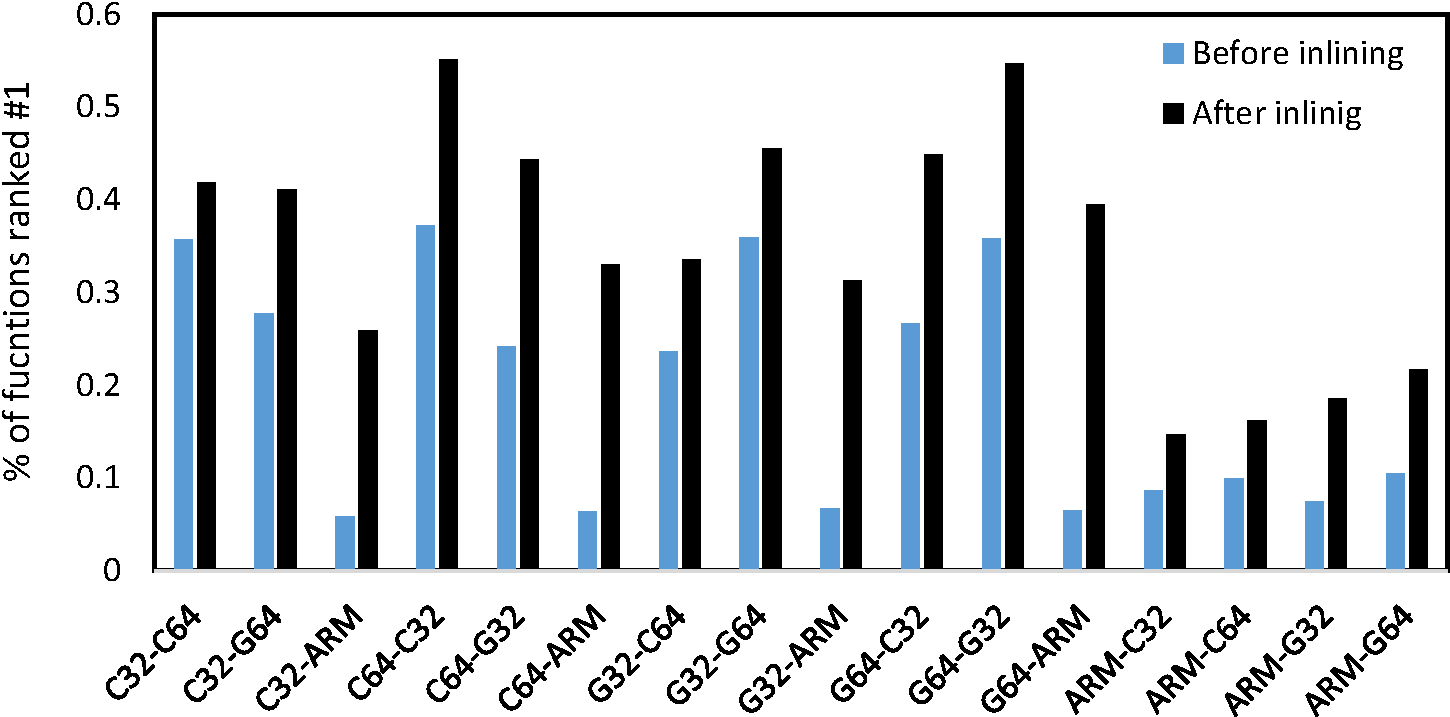
\includegraphics[height=4cm]{srj-figures/srj-cross-archi.pdf} %\vspace{-1mm}
\caption{In \tool, cross-architecture function matching before/after selective inlining using \texttt{coreutils} binaries. Here, \textbf{C} and \textbf{G} represent  compilers \texttt{clang} and \texttt{gcc}, respectively, and 32 and 64 denote x86 32bit and 64bit architectures. }
\label{fig:cross-archi}

\end{center}
\end{figure}


%\noindent\textbf{Cross-architecture analysis.}
%\textbf{Answer to RQ1.a: Cross-architecture analysis.}\label{sec:expe:rq1_a}
\subsubsection{\tool's Answer to RQ1}\label{sec:evaluation_rq1.1}
We conduct two experiments. First experiment is to match all functions in \texttt{coreutils} binaries compiled for one architecture (i.e., x86 32bit, x86 64bit and ARM) to the semantically equivalent functions in binaries compiled for another architecture. For example, binaries compiled for ARM are matched against the binaries compiled for x86 32bit and x86 64bit architectures, and \emph{vice versa}.  In all three architectures, the compilation uses \texttt{gcc} (v4.8.2) and \texttt{clang} (v3.0) with the optimization level \texttt{O2} (default settings in many Linux distributions).

Fig.~\ref{fig:cross-archi} summarizes the average results (before and after selective inlining) obtained for \texttt{coreutils} binaries, where we report the percentage of functions ranked one (i.e., best match).
%in the matching.
In the plot,  the bar \texttt{G64-G32} (after inlining) should be read as, when functions compiled, using \texttt{gcc}, for x86 64bit architecture are used as signature, around 55\% of the functions compiled, using \texttt{gcc}, for x86 32bit architecture achieve rank one. It is observed that when ARM binary functions are used as signatures, the overall results significantly degrade --- only 18\% of the functions are ranked one, compare to x86 32bit and 64bit architectures, where it is around 41\%.
%Table \ref{tab:cross-arch-with-behav} summarizes the results for 14 largest \texttt{coreutils} binaries (e.g., \texttt{cp}, \texttt{df}, $\ldots$) and the last row shows the averages for rest of the 89 binaries . It can be seen that on average 18\% of the functions in the largest 14 binaries are ranked 1, this increases to 30.4\% for rest of the binaries. Further, around 71\% of the large binaries are ranked within top 5 positions, where it is 82\% for other small binaries.
We also notice that matching(after inlining) between binaries compiled for ARM and x86 64bit  yields higher ranking compared to ARM and x86 32bit binaries. The rationale is that ARM and x86 64bit binaries are register intensive compared to x86 32bit binaries ---  in ARM and x86 64bit architectures, there are 16 general-purpose registers, and hence registers are used more frequently than used in x86 32bit binaries which have only 8.

%However, the \texttt{coreutils} binaries are relatively small with around 100-150 functions (on avg.) per binary. Hence, to compare the robustness of \tool in larger binaries with several thousand functions, we repeated the experiment with \texttt{BusyBox} (v1.21.1), where functions in x86 32bit, x86 62bit and ARM are matched against each other.
%From Table \ref{tab:x86_x64_box},
Considering the fact that \texttt{coreutils} binaries are relatively small with around 250 functions (on average) per binary, we conduct the second experiment using \texttt{BusyBox} (v1.21.1), which contains 2,410 functions.
%\xyx{Considering the relatively small size of functions (100-150) in \texttt{coreutils}, we conduct the same experiment on the second case \texttt{BusyBox} (v1.21.1) which contains 2410 functions.}
We observe that the obtained results are comparable with the results of \texttt{coreutils} binaries --- 41.3\% of the functions are best-match in \texttt{BusyBox}, while it is 35\% for \texttt{coreutils} binaries on average across 16 experiments shown in Fig.~\ref{fig:cross-archi}. This is an improvement of 27.5\% over the accuracy achieved by~\cite{DBLP:conf/sp/PewnyGGRH15} for \texttt{BusyBox}.
However, for top-10 match (i.e., ranking 1-10), \texttt{coreutils} binaries achieve better results than \texttt{BusyBox} (78.4\% vs. 67\%). This result might be due to function size of the binary --- in \texttt{BusyBox}, a function needs to be compared against on average 3,250 functions, and in \texttt{coreutils} binaries around 250  functions need to be compared. %This illustrates the robustness of \tool across architectures.\\

\begin{table}[t]
\scriptsize
\centering
\caption{Total no. of functions selectively inlined in \texttt{coreutils} binaries compiled using \texttt{gcc} and \texttt{clang} for ARM, x86 32bit and 64bit architectures. }
\label{cross-archi-inline}
\begin{tabular}{@{}llllll@{}}
\toprule
                                         & ARM                        & C64                        & G64                        & C32                        & G32                        \\ \midrule
\multicolumn{1}{l|}{Total functions}     & \multicolumn{1}{l|}{27,820} & \multicolumn{1}{l|}{23,782} & \multicolumn{1}{l|}{24,489} & \multicolumn{1}{l|}{24,002} & \multicolumn{1}{l|}{24,792} \\ \cmidrule(l){2-6}
%\multicolumn{1}{l|}{Candidate functions} & \multicolumn{1}{l|}{4251}  & \multicolumn{1}{l|}{2260}  & \multicolumn{1}{l|}{2671}  & \multicolumn{1}{l|}{2464}  & \multicolumn{1}{l|}{3295}  \\ \cmidrule(l){2-6}
\multicolumn{1}{l|}{Inlined functions}   & \multicolumn{1}{l|}{1,620}  & \multicolumn{1}{l|}{776}   & \multicolumn{1}{l|}{1,002}  & \multicolumn{1}{l|}{823}   & \multicolumn{1}{l|}{1,188}  \\ \bottomrule
\end{tabular}
\end{table}


\noindent\textbf{Impact of selective inlining.} As shown in Fig.~\ref{fig:cross-archi}, our selective inlining significantly improves the overall matching accuracy by 150\% on average. In particular, when ARM architecture is used as target, selective inlining improves the total matching accuracy on average by about 400\%. Table~\ref{cross-archi-inline} summarizes the total number of functions inlined for each architecture.  We notice that \texttt{coreutils} compiled for ARM contains more functions (27,820 across 103 binaries) than that compiled for x86 32bit (avg. 24,397) and x86 64bit (avg. 24,136). From the second row of Table~\ref{cross-archi-inline}, it can be seen that 61\% and 82\% more functions are selectively inlined by \tool in ARM than that in x86 32bit and 64bit architectures, respectively. In ARM binaries, the larger number of compiled functions suggests that compiler inlining does not happen as frequently as it does in the other two architectures.  Hence,   selective inlining is required to capture the complete semantics in binary analysis, which results in the improved matching accuracy.

\noindent\textbf{Summary.} On \texttt{coreutils} and \texttt{BusyBox} binaries, \tool achieves the best match (i.e., rank \#1) for 35\%-42\% of the functions on average, for cross-architecture analysis, and selective inlining improves the result by 150\% on average.

\subsubsection{\toolNew's Answer to RQ1}\label{sec:evaluation_rq1.2}

\begin{figure}[t]
\begin{center}%\vspace{-3mm}
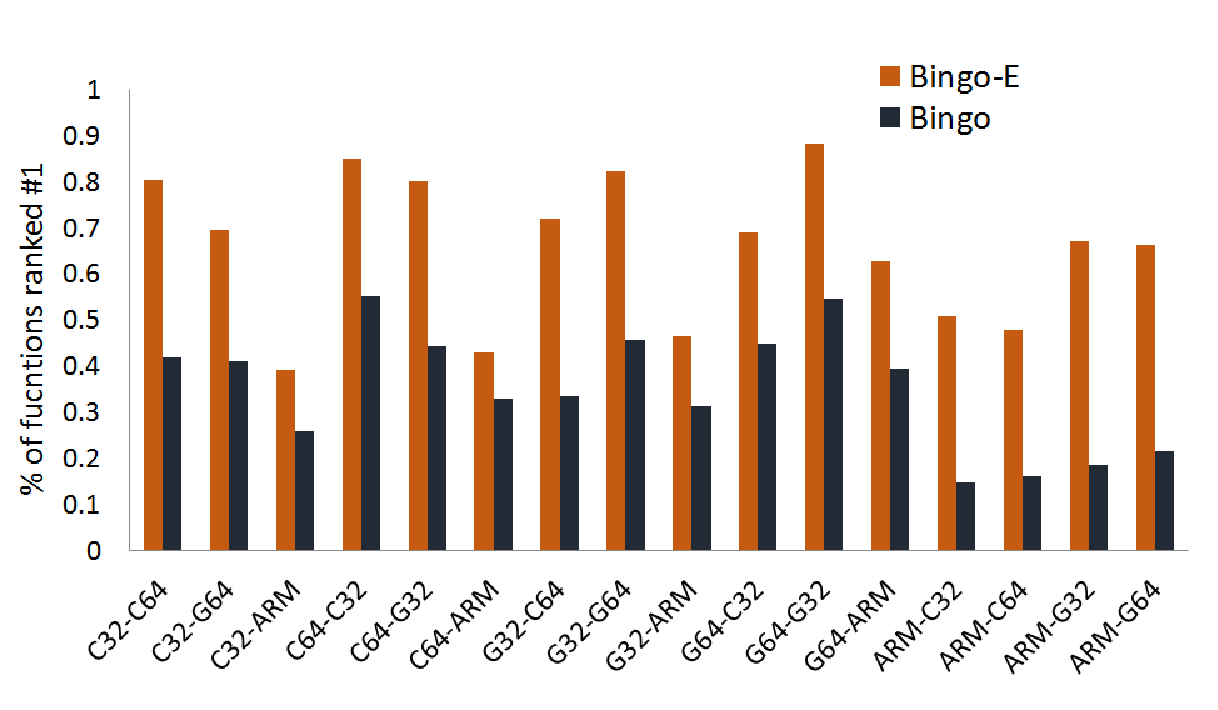
\includegraphics[height=5cm]{srj-figures/cross-archi-new.pdf} %\vspace{-1mm}
\caption{Cross-architecture function matching after selective inlining using \texttt{coreutils} binaries for \tool and \toolNew. Here, \textbf{C} and \textbf{G} represent  compilers \texttt{clang} and \texttt{gcc}, respectively, and 32 and 64 denote x86 32bit and 64bit architectures. }
\label{fig:cross-archi-new}
\end{center}
\end{figure}


For \toolNew, we also match the binary functions in \texttt{coreutils} binaries compiled for one architectures (i.e., x86 32bit, x86 64bit and ARM) to that for another. We use the two compilers \texttt{gcc} (v4.8.2) and \texttt{clang} (v3.0) with the optimization level \texttt{O2} (default settings in many Linux distributions). %Hence, the setup of the experiment is the same as that in \S~\ref{subsec:robut}.

Fig.~\ref{fig:cross-archi-new} shows the average results after selective inlining on \texttt{coreutils} binaries for \tool and \toolNew.
Note we only count the percentage of functions ranked 1st (i.e., best match in the case of mapping the binary functions from the same source code).
In Fig.~\ref{fig:cross-archi-new}, we list 16 possible scenarios of cross-architecture code matching.
For example, in the plot, the brown bar \texttt{G64-ARM}  denotes the result that 62.7\% of the functions (signatures) compiled by \texttt{gcc}  for  x86-64 are the best matches of those functions (targets) compiled by \texttt{gcc} for ARM architecture according to \toolNew.

Previously, we observed that in Fig.~\ref{fig:cross-archi} that when  binary functions compiled for ARM are used as signatures, the  matching results significantly degrade --- only 18\% of the functions are ranked 1st, based on the low-level semantic features in \tool. \xyx{The reason is that  I/O values of registers in \tool are not effective for cross-architecture matching.} Hence, in \toolNew, the newly added high-level semantic and structural features are complement to improve the matching accuracy. The results in Fig.~\ref{fig:cross-archi-new} prove the effectiveness of these new features. For most cases, the new features improve the matching accuracy by at least 50\%, compared to the results of \tool. Especially, in the cases of code for ARM as signatures (\texttt{ARM-C32}, \texttt{ARM-C64}, \texttt{ARM-G32}, \texttt{ARM-G64}), the improvement of best match rate is above 200\%. This indicates the ineffectiveness of low-level semantic features used by \tool for matching the code for ARM to the code for other architectures.


%Only in the cases of code for ARM as targets (\texttt{C32-ARM}, \texttt{C64-ARM} and \texttt{G32-ARM}), the improvement is less than 50\%.
\xyx{Currently, for \toolNew, we get more similar results for many cases --- the best match rate is within the range of  $70\% \sim 90\%$ for  the mapping from x86-32 to x86-64 (or the other way around), while the  best match rate drops to  $40\% \sim 60\%$ if the ARM code is used as signatures or targets. The rationale is that the BB structure of code for x86-32 or x86-64 is highly similar; even in code for ARM, the basic BB structure is also retained during the cross-architecture compilation.
Hence, the structural features and high-level semantic features are the effective complements, since the CFG structures and function call information are retained during the compilation (no matter we use \texttt{gcc}  or \texttt{clang}). We find that the high-level semantic features, if  they are available, are even more helpful than structural features. The reason is that after selective inlining the information on function call in binary code does not change with the compilation options of architecture.}

Another interesting observation is that the results for \toolNew are much more symmetric than the results of \tool. For example, the best match rate for \toolNew in \texttt{C64-ARM} and \texttt{ARM-C64} is 0.431 and 0.479, respectively. Hence, reversing signatures and targets does not affect as much as that in \tool. In contrast,  for \tool in \texttt{C64-ARM} and \texttt{ARM-C64} it is 0.33 and 0.162, respectively. The unsymmetrical results for \tool are due to the step of function model generation, in which $k$-tracelet is sampled and generated from the CFG. As applying graph isomorphism for CFG matching, the matching of CFG $g_1$ to $g_2$ does not mean the matching of $g_2$ to $g_1$ --- $g_1$ may be a sub-graph of $g_2$ and using $g_2$ as signatures leads to a similarity score lower than the similarity threshold. Similarly, in \tool, low level semantic features extracted from $k$-tracelet (i.e., sampled partial CFG) also have this issue of unsymmetrical results.

To mitigate this, the function similarity  (i.e., FDD in \S~\ref{sec:category:structralFea}) for 3D-CFG is defined to produce symmetrical results, according to Definition 3. In addition, the high-level semantic features (e.g., function call information) are retained in cross-architecture compilation. Hence, the results of \toolNew are more symmetrical than that of \tool.

%Nevertheless, when the ARM code is used as targets, the structural features are less effective than they are when the code for e x86-32 or x86-64  is targets. %\xyx{After a  scrutiny of the matching results, we observe that,  after the compilation of the source code, the code for ARM seems to have simpler BB structure than that for x86-32 or x86-64. Accord to the 3D-CFG features,  }
%Table \ref{tab:cross-arch-with-behav} summarizes the results for 14 largest \texttt{coreutils} binaries (e.g., \texttt{cp}, \texttt{df}, $\ldots$) and the last row shows the averages for rest of the 89 binaries . It can be seen that on average 18\% of the functions in the largest 14 binaries are ranked 1, this increases to 30.4\% for rest of the binaries. Further, around 71\% of the large binaries are ranked within top 5 positions, where it is 82\% for other small binaries.

%We also notice that matches (after inlining) between binaries compiled for ARM and x86 64bit  yield higher ranking compared to ARM and x86 32bit binaries. The rationale is that ARM and x86 64bit binaries are register intensive compared to x86 32bit binaries ---  in ARM and x86 64bit architectures, there are 16 general-purpose registers, and hence registers are used more frequently than used in x86 32bit binaries which have only 8.

\vspace{2mm}
\noindent\fbox{\parbox{1\linewidth}{In this experiment, on average, our approach significantly improves the accuracy of best match rate from 35.1\% (for \tool) to 65.6\% (for \toolNew) on \texttt{coreutils}.  For cross-architecture matching on the same code base, structural features and high-level semantic features are effective, being good complement to low-level semantic features. Further, \toolNew's results are more symmetrical than \tool's.}  }


%\begin{table}[ht]
%\caption{Percentage of functions ranked \#1 in intra-compiler (x86 64bit) comparison. Here, \textbf{G} and \textbf{G'} represent \texttt{gcc} v4.8.3 and v4.6 compilers, respectively.}
%\begin{minipage}{.5\linewidth}
%
%\scriptsize
%
%\label{my-label}
%\begin{tabular}{@{}lllll@{}}
%                        & G0                        & G1                        & G2                        & G3                        \\ \cmidrule(l){2-5}
%\multicolumn{1}{l|}{G'0} & \multicolumn{1}{l|}{0.45} & \multicolumn{1}{l|}{0.37} & \multicolumn{1}{l|}{0.41} & \multicolumn{1}{l|}{0.25} \\ \cmidrule(l){2-5}
%\multicolumn{1}{l|}{G'1} & \multicolumn{1}{l|}{0.37} & \multicolumn{1}{l|}{0.47} & \multicolumn{1}{l|}{0.51} & \multicolumn{1}{l|}{0.32} \\ \cmidrule(l){2-5}
%\multicolumn{1}{l|}{G'2} & \multicolumn{1}{l|}{0.47} & \multicolumn{1}{l|}{0.54} & \multicolumn{1}{l|}{0.57} & \multicolumn{1}{l|}{0.47} \\ \cmidrule(l){2-5}
%\multicolumn{1}{l|}{G'3} & \multicolumn{1}{l|}{0.37} & \multicolumn{1}{l|}{0.44} & \multicolumn{1}{l|}{0.52} & \multicolumn{1}{l|}{0.54} \\ \cmidrule(l){2-5}
%\end{tabular}
%\end{minipage}%
%\begin{minipage}{.5\linewidth}
%
%\scriptsize
%
%\label{my-label}
%\begin{tabular}{@{}lllll@{}}
%                        & G'0                        & G'1                        & G'2                        & G'3                        \\ \cmidrule(l){2-5}
%\multicolumn{1}{l|}{G0} & \multicolumn{1}{l|}{0.45} & \multicolumn{1}{l|}{0.36} & \multicolumn{1}{l|}{0.41} & \multicolumn{1}{l|}{0.34} \\ \cmidrule(l){2-5}
%\multicolumn{1}{l|}{G1} & \multicolumn{1}{l|}{0.39} & \multicolumn{1}{l|}{0.49} & \multicolumn{1}{l|}{0.52} & \multicolumn{1}{l|}{0.39} \\ \cmidrule(l){2-5}
%\multicolumn{1}{l|}{G2} & \multicolumn{1}{l|}{0.44} & \multicolumn{1}{l|}{0.55} & \multicolumn{1}{l|}{0.59} & \multicolumn{1}{l|}{0.53} \\ \cmidrule(l){2-5}
%\multicolumn{1}{l|}{G3} & \multicolumn{1}{l|}{0.3}  & \multicolumn{1}{l|}{0.39} & \multicolumn{1}{l|}{0.51} & \multicolumn{1}{l|}{0.51} \\ \cmidrule(l){2-5}
%\end{tabular}
%\end{minipage}%
%\end{table}


%\begin{table}[t]
%\scriptsize
%\centering
%\caption{Rankings (top 10 matches) obtained by \tool for 60 functions in \texttt{msvcrt} against \texttt{libc}}
%\label{tab:cross-os}
%\begin{tabular}{@{}lll@{}}
%\multicolumn{1}{c}{\textbf{Rank}}    & \multicolumn{1}{c}{\textbf{Library functions}}   & \#                       \\ \cmidrule(l){1-3}
%\multicolumn{1}{l|}{1}      & \multicolumn{1}{l|}{\parbox{6cm}{tolower, memset, wcschr, wcsncmp, toupper, memcmp, strspn, wcsrchr, memchr, strrch,r strchr}}                                                              & \multicolumn{1}{l}{11}  \\ \cmidrule(l){1-3}
%\multicolumn{1}{l|}{2-3}    & \multicolumn{1}{l|}{\parbox{6cm}{wcstoul, wcstol, strtoul, fopen, strncpy, strtol, itoa, wcscmp, wcsncat, itow, longjmp, strcspn, wcsncpy, labs, strpbrk, toupper, write, memcpy, memmove, tolower}} & \multicolumn{1}{l}{20} \\ \cmidrule(l){1-3}
%\multicolumn{1}{l|}{4-5}    & \multicolumn{1}{l|}{\parbox{6cm}{mbtowc, wcstombs, strcat, remove, mbstowcs, wctomb}}                                                                                                   & \multicolumn{1}{l}{6}  \\ \cmidrule(l){1-3}
%\multicolumn{1}{l|}{6-10}   & \multicolumn{1}{l|}{\parbox{6cm}{rename, strstr, wcspbrk, iswctype, strtok, wcscoll, strcoll, setlocale, qsort, wcsspn, swprintf, wcstod, strerrorr}}                                         & \multicolumn{1}{l}{13}  \\ \cmidrule(l){1-3}
%%\multicolumn{1}{l|}{11-20}  & \multicolumn{1}{l|}{\parbox{6cm}{strncat, raise, strtod, wcscspn, wcstok, atol}}                                                                                                        & \multicolumn{1}{l|}{6}  \\ \cmidrule(l){1-3}
%%\multicolumn{1}{l|}{21-50}  & \multicolumn{1}{l|}{perror, system, wcsxfrm}                                                                                                                           & \multicolumn{1}{l|}{3}   \\ \cmidrule(l){1-3}
%%\multicolumn{1}{l|}{51-100} & \multicolumn{1}{l|}{strxfrm}                                                                                                                                           & \multicolumn{1}{l|}{1}      \\ \cmidrule(l){1-3}
%\end{tabular}\vspace{-1mm}
%\end{table}

%\noindent\textbf{Cross-compiler analysis.}

\subsection{Answer to RQ2: Robustness in Cross-compiler Matching}\label{sec:evaluation_rq2}
\subsubsection{\tool's Answer to RQ2}

\textbf{Inter-compiler Matching.} Table~\ref{tab:cross-comp-inter} summarizes the results obtained by \tool for different compilers (\texttt{gcc} and \texttt{clang}) with various optimization levels (O0, O1, O2 and O3) for x86 32bit architecture.
Here, each row and column of the table represents the compiler (including the level of optimization) used to compile the signature and target functions, respectively.
%functions while each column denotes the compiler used to compile the target functions.
For example, the cell denoted by the second row and fifth column (\texttt{C1G0}) represents the result for which signature functions are compiled using \texttt{clang}  with optimization level \texttt{O1} and the target functions are compiled using \texttt{gcc} with  \texttt{O0}.
From the table, we observe that \tool is good, %in most cases (except when  \texttt{gcc\_O3} is used as a signature)
as 41.5\% of the functions achieve rank one (on average across all the experiments for binaries compiled for x86 32bit) while this increases to 84\% for top 10 matches, which is very promising. We observed similar behaviour in binaries compiled for x86 64bit architecture and due to space constraints, the results are reported in our tool webpage~\cite{bingo@fse2016}.% Further, we also report the individual results obtained by each of these 103 binaries (e.g., \texttt{ls}, \texttt{true}, and so on) in the \texttt{coretuils} suite, for every experiment, in~\cite{bingo@fse2016}.
%In addition, during cross-compiler analysis, if no optimization is used in either one of the side, the obtained rankings are relatively low compare to optimized binaries, this observation is inlined with~\cite{DBLP:conf/sp/PewnyGGRH15}.

Interestingly, we find that regardless of the compiler type, matches between the binaries that are compiled with high code optimization levels (i.e., \texttt{O2} and \texttt{O3}) yield better results than matches between binaries with no code optimization (i.e.,\texttt{O0}). That is, high code optimization levels lead to the similar binary code even with different compilers, whereas without optimization the  influence of the compiler in the binary is very evident. This observation is consistent with~\cite{DBLP:conf/sp/PewnyGGRH15}. Further, within one compiler type (e.g., \texttt{gcc}), the matching accuracy achieved by optimization level \texttt{O2}, across all other compiler types and optimization levels, is always better or consistent with the results obtained by \texttt{O3} (relevant rows are shaded in light gray in Table~\ref{tab:cross-comp-inter}). This behaviour is observed in x86 64bit architecture too.


\noindent\textbf{Intra-compiler Matching.} In addition, we also conduct the experiments across different versions of the same compiler (\texttt{gcc} v4.8.3 vs. \texttt{gcc} v4.6) and the results (for x86 32bit architecture) are summarized in Table~\ref{tab:cross-comp-intra}.
%The observations are pretty similar to the inter-compiler analysis, where the comparisons against optimized code, in general, achieve better accuracy while the comparisons against unoptimized code weakens the matching accuracy.
%Interestingly,  it is observed that when functions compiled with optimization level \texttt{O1} are used as signatures, functions compiled with optimization level \texttt{O2} yield better accuracy, except when \texttt{gcc} v4.8.3 is used to compile the signature binaries for x86 32bit architecture.
%For all other cases,
As expected, the highest accuracy is achieved when the signature and target functions are of the same optimization level, except when the signature functions are compiled with optimization level \texttt{O1}, where on such occasions, target functions compiled with optimization level \texttt{O2} yield better accuracy. The best results obtained for each signature binary is highlighted in light gray in Table~\ref{tab:cross-comp-intra}.
Further, we also observe that the overall accuracy for intra-compiler analysis (42.7\%) is slightly better than the inter-compiler analysis (41.5\%). %where 43.6\% (overall average) of the functions achieved rank one in intra-compiler analysis, a 5.5\% improvement.
Finally, in intra-compiler analysis, around 76.3\% functions ranked within top 5 positions, whereas it is only 68.5\% for inter-compiler analysis, an 11.8\% improvement. Details on the results of intra-compiler analysis for x86 64bit architecture are reported in~\cite{bingo@fse2016}.
%within same compilers, better ranks are achieved when the functions are matched from optimization level O3 to O0 (i.e., highest to no optimization) and the worst ranks are achieved when the matching is inverted, i.e., from O0 to O3. This could be attributed to the fact that in O3 the compiler merges as many functions as possible, using function inlining, and makes the functions very compact. Hence, for one function in O3 there may be many semantically similar functions in O0, where there is no optimization at all (i.e.,\textit{ 1-to-n} matching). However, on the other hand, for several functions in O0 there will be only one function in O3 which may be semantically less similar to all of them individually (i.e., \textit{n-to-1} matching). This behavior is not particular to certain compiler as its observed both in \texttt{gcc} and \texttt{clang} compilers.

\noindent\textbf{Impact of selective inlining.}  We observe that selective inlining improves the average matching accuracy by around 140\% for cross-compiler analysis. Many functions are inlined when the binaries are compiled with the optimization level \texttt{O0} compared to \texttt{O3}. In particular, 1,473 functions (on average across \texttt{gcc} and \texttt{clang}) are inlined in for optimization level \texttt{O0}, whereas, it is only 831 for \texttt{O3}.

\noindent\textbf{Summary.} %On \texttt{coreutils} and \texttt{BusyBox} binaries, \tool achieves the best match (i.e., rank \#1) for 35\%-42\% of the functions on average, for cross-architecture analysis, and selective inlining improves the result by 150\% on average.
For different types and versions of compiler, in most cases, \tool attains the best match for around 42\% of the functions, and top-5 match for around 72\% of the functions on average.

\begin{table}[t]
\scriptsize
\centering
\caption{In \tool, percentage of functions ranked \#1 in inter-compiler (x86 32bit) comparison for \texttt{coreutils}. Here, \textbf{C} and \textbf{G} represent \texttt{clang} and \texttt{gcc} compilers, respectively and 0-3 represents optimization O0-O3. }
\label{tab:cross-comp-inter}
\begin{tabular}{@{}lllllllll@{}}
\textbf{} & \textbf{C0} & \textbf{C1} & \textbf{C2} & \textbf{C3} & \textbf{G0} & \textbf{G1} & \textbf{G2} & \textbf{G3} \\ \cmidrule(l){2-9}
\multicolumn{1}{l|}{\textbf{C0}} & \multicolumn{1}{c|}{-} & \multicolumn{1}{l|}{0.402} & \multicolumn{1}{l|}{0.373} & \multicolumn{1}{l|}{0.372} & \multicolumn{1}{l|}{0.371} & \multicolumn{1}{l|}{0.4} & \multicolumn{1}{l|}{0.451} & \multicolumn{1}{l|}{0.332} \\ \cmidrule(l){2-9}
\multicolumn{1}{l|}{\textbf{C1}} & \multicolumn{1}{l|}{0.392} & \multicolumn{1}{c|}{-} & \multicolumn{1}{l|}{0.456} & \multicolumn{1}{l|}{0.455} & \multicolumn{1}{l|}{0.396} & \multicolumn{1}{l|}{0.429} & \multicolumn{1}{l|}{0.503} & \multicolumn{1}{l|}{0.388} \\ \cmidrule(l){2-9}
\multicolumn{1}{l|}{\textbf{C2}} & \multicolumn{1}{l|}{\cellcolor[HTML]{EFEFEF}0.345} & \multicolumn{1}{l|}{\cellcolor[HTML]{EFEFEF}0.426} & \multicolumn{1}{c|}{\cellcolor[HTML]{EFEFEF}-} & \multicolumn{1}{l|}{\cellcolor[HTML]{EFEFEF}0.576} & \multicolumn{1}{l|}{\cellcolor[HTML]{EFEFEF}0.344} & \multicolumn{1}{l|}{\cellcolor[HTML]{EFEFEF}0.411} & \multicolumn{1}{l|}{\cellcolor[HTML]{EFEFEF}0.488} & \multicolumn{1}{l|}{\cellcolor[HTML]{EFEFEF}0.478} \\ \cmidrule(l){2-9}
\multicolumn{1}{l|}{\textbf{C3}} & \multicolumn{1}{l|}{0.344} & \multicolumn{1}{l|}{0.425} & \multicolumn{1}{l|}{0.575} & \multicolumn{1}{c|}{-} & \multicolumn{1}{l|}{0.343} & \multicolumn{1}{l|}{0.41} & \multicolumn{1}{l|}{0.488} & \multicolumn{1}{l|}{0.477} \\ \cmidrule(l){2-9}
\multicolumn{1}{l|}{\textbf{G0}} & \multicolumn{1}{l|}{0.344} & \multicolumn{1}{l|}{0.354} & \multicolumn{1}{l|}{0.334} & \multicolumn{1}{l|}{0.333} & \multicolumn{1}{c|}{-} & \multicolumn{1}{l|}{0.374} & \multicolumn{1}{l|}{0.398} & \multicolumn{1}{l|}{0.302} \\ \cmidrule(l){2-9}
\multicolumn{1}{l|}{\textbf{G1}} & \multicolumn{1}{l|}{0.37} & \multicolumn{1}{l|}{0.409} & \multicolumn{1}{l|}{0.41} & \multicolumn{1}{l|}{0.409} & \multicolumn{1}{l|}{0.376} & \multicolumn{1}{c|}{-} & \multicolumn{1}{l|}{0.517} & \multicolumn{1}{l|}{0.395} \\ \cmidrule(l){2-9}
\multicolumn{1}{l|}{\textbf{G2}} & \multicolumn{1}{l|}{\cellcolor[HTML]{EFEFEF}0.412} & \multicolumn{1}{l|}{\cellcolor[HTML]{EFEFEF}0.462} & \multicolumn{1}{l|}{\cellcolor[HTML]{EFEFEF}0.474} & \multicolumn{1}{l|}{\cellcolor[HTML]{EFEFEF}0.473} & \multicolumn{1}{l|}{\cellcolor[HTML]{EFEFEF}0.428} & \multicolumn{1}{l|}{\cellcolor[HTML]{EFEFEF}0.514} & \multicolumn{1}{c|}{\cellcolor[HTML]{EFEFEF}-} & \multicolumn{1}{l|}{\cellcolor[HTML]{EFEFEF}0.48} \\ \cmidrule(l){2-9}
\multicolumn{1}{l|}{\textbf{G3}} & \multicolumn{1}{l|}{0.326} & \multicolumn{1}{l|}{0.372} & \multicolumn{1}{l|}{0.438} & \multicolumn{1}{l|}{0.439} & \multicolumn{1}{l|}{0.331} & \multicolumn{1}{l|}{0.42} & \multicolumn{1}{l|}{0.5} & \multicolumn{1}{c|}{-} \\ \cmidrule(l){2-9}
\end{tabular}
\end{table}



\begin{table}[t]
%\vspace{5mm}
\caption{In \tool, percentage of functions ranked \#1 in intra-compiler (x86 32bit) comparison for \texttt{coreutils}. Here, \textbf{G} and \textbf{G'} represent \texttt{gcc} v4.8.3 and v4.6 compilers, respectively.}
\label{tab:cross-comp-intra}
\begin{minipage}{.5\linewidth}
\scriptsize
\begin{tabular}{@{}lllll@{}}
                        & G0                        & G1                        & G2                        & G3                        \\ \cmidrule(l){2-5}
\multicolumn{1}{l|}{G'0} & \multicolumn{1}{l|}{\cellcolor[HTML]{EFEFEF}0.43} & \multicolumn{1}{l|}{0.36} & \multicolumn{1}{l|}{0.36} & \multicolumn{1}{l|}{0.27} \\ \cmidrule(l){2-5}
\multicolumn{1}{l|}{G'1} & \multicolumn{1}{l|}{0.37} & \multicolumn{1}{l|}{0.46} & \multicolumn{1}{l|}{\cellcolor[HTML]{EFEFEF}0.48} & \multicolumn{1}{l|}{0.36} \\ \cmidrule(l){2-5}
\multicolumn{1}{l|}{G'2} & \multicolumn{1}{l|}{0.4}  & \multicolumn{1}{l|}{0.44} & \multicolumn{1}{l|}{\cellcolor[HTML]{EFEFEF}0.52} & \multicolumn{1}{l|}{0.41} \\ \cmidrule(l){2-5}
\multicolumn{1}{l|}{G'3} & \multicolumn{1}{l|}{0.4}  & \multicolumn{1}{l|}{0.44} & \multicolumn{1}{l|}{0.49} & \multicolumn{1}{l|}{\cellcolor[HTML]{EFEFEF}0.49} \\ \cmidrule(l){2-5}
\end{tabular}
\end{minipage}%
\begin{minipage}{.5\linewidth}

\scriptsize

\begin{tabular}{@{}lllll@{}}
                        & G'0                        & G'1                        & G'2                        & G'3                        \\ \cmidrule(l){2-5}
\multicolumn{1}{l|}{G0} & \multicolumn{1}{l|}{\cellcolor[HTML]{EFEFEF}0.44} & \multicolumn{1}{l|}{0.4}  & \multicolumn{1}{l|}{0.41} & \multicolumn{1}{l|}{0.42} \\ \cmidrule(l){2-5}
\multicolumn{1}{l|}{G1} & \multicolumn{1}{l|}{0.38} & \multicolumn{1}{l|}{0.47} & \multicolumn{1}{l|}{\cellcolor[HTML]{EFEFEF}0.48} & \multicolumn{1}{l|}{0.45} \\ \cmidrule(l){2-5}
\multicolumn{1}{l|}{G2} & \multicolumn{1}{l|}{0.4}  & \multicolumn{1}{l|}{0.49} & \multicolumn{1}{l|}{\cellcolor[HTML]{EFEFEF}0.52} & \multicolumn{1}{l|}{0.5}  \\ \cmidrule(l){2-5}
\multicolumn{1}{l|}{G3} & \multicolumn{1}{l|}{0.32} & \multicolumn{1}{l|}{0.39} & \multicolumn{1}{l|}{0.43} & \multicolumn{1}{l|}{\cellcolor[HTML]{EFEFEF}0.52} \\ \cmidrule(l){2-5}
\end{tabular}
\end{minipage}\vspace{0mm}%
\end{table}

\subsubsection{\toolNew's answer to RQ2}

\textbf{Inter-compiler Matching.} Still using \texttt{coreutils} binaries, Table \ref{tab:new_cross-comp-inter} summarizes the results obtained by \toolNew for different compilers (gcc and clang) with various optimization levels (O0, O1, O2 and O3) on  \texttt{coreutils} for x86 32bit architecture. The row represents the optimization level of signature functions and the column represents that of target functions. We observe that the best results are usually achieved when O1 or O2 is adopted. The worst results (below 80\%) are achieved when O3 is used, no matter for \texttt{gcc} or \texttt{clang}. Even C2-to-G1 or G2-to-C1 can achieve an accuracy above 88\%. Hence, for cross-compiler matching, we find the impact of compiler differences matters less than that of the optimization levels.

\vspace{2mm}
\noindent\fbox{\parbox{1\linewidth}{In this experiment, \toolNew (best-match rate ranging from 70.1\% to 99.7\% in Table \ref{tab:new_cross-comp-inter}) exhibits significant improvement over \tool (best-match rate ranging from 32\% to 58\% in Table \ref{tab:cross-comp-inter}) for cross-compiler analysis. The improvement is attributed to the use of features of BB structure and high-level semantics, as BB structure can be retained for different compilers under the same or similar optimization levels.}}

\vspace{2mm}

\textbf{Intra-compiler Matching.} We also conduct intra-compiler matching for \toolNew. Table~\ref{tab:new_cross-comp-intra} summarizes the searching results obtained by \toolNew for differen versions of the compiler \texttt{gcc} with various optimization levels (O0, O1, O2 and O3) for x86 32bit architecture. Here, each row and column of the table represents the compiler (including the level of optimization) used to compile the signature and target functions, respectively. For example, for the cell at row G'0 and column G0 in the left part of Table~\ref{tab:new_cross-comp-intra}, the value 0.91 means that 91\% of functions successfully match if we use the version compiled by G'0 as signature and use the function compiled  by G0 as target. It can be observed that usually the best-match results are achieved when the signature and target functions are combined by the same optimization level (O0-O2, except O3). The reasons lie that \toolNew adopts the structural and high-level semantic features for intra and cross compiler matching. When the same optimization level (except O3) is used for signature and target functions, the structural information is well-retained. However, when O3 is used, the structure of the binary is so over-optimized that less information is retained for structural matching. The two over-optimized program may have less structural similarity in G'3-to-G3 or G3-to-G'3 matching.

\vspace{2mm}
\noindent\fbox{\parbox{1\linewidth}{In the experiment, the results of \toolNew (best-match rate ranging from 70\% to 98\% in Table \ref{tab:new_cross-comp-intra}) are significantly better than the results of \tool (best-match rate ranging from 27\% to 52\% in  Table \ref{tab:cross-comp-intra}). For the same code base with intra-compiler matching, the structural and high-level semantic features are more effective than the low-level semantic features, relying on the retained structural information. }}



\begin{table}[t]
\scriptsize
\centering
\caption{In \toolNew, percentage of functions ranked \#1 in inter-compiler (x86 32bit) comparison for \texttt{coreutils}. Here, \textbf{C} and \textbf{G} represent \texttt{clang} and \texttt{gcc} compilers, respectively and 0-3 represents optimization O0-O3. }
\label{tab:new_cross-comp-inter}
\begin{tabular}{@{}lllllllll@{}}
\textbf{} & \textbf{C0} & \textbf{C1} & \textbf{C2} & \textbf{C3} & \textbf{G0} & \textbf{G1} & \textbf{G2} & \textbf{G3} \\ \cmidrule(l){2-9}
\multicolumn{1}{l|}{\textbf{C0}} & \multicolumn{1}{c|}{-} & \multicolumn{1}{l|}{0.865} & \multicolumn{1}{l|}{0.791} & \multicolumn{1}{l|}{0.785} & \multicolumn{1}{l|}{0.799} & \multicolumn{1}{l|}{0.840} & \multicolumn{1}{l|}{0.836} & \multicolumn{1}{l|}{0.701} \\ \cmidrule(l){2-9}
\multicolumn{1}{l|}{\textbf{C1}} & \multicolumn{1}{l|}{0.840} & \multicolumn{1}{c|}{-} & \multicolumn{1}{l|}{0.838} & \multicolumn{1}{l|}{0.833} & \multicolumn{1}{l|}{0.891} & \multicolumn{1}{l|}{0.913} & \multicolumn{1}{l|}{0.887} & \multicolumn{1}{l|}{0.756} \\ \cmidrule(l){2-9}
\multicolumn{1}{l|}{\textbf{C2}} & \multicolumn{1}{l|}{\cellcolor[HTML]{EFEFEF}0.814} & \multicolumn{1}{l|}{\cellcolor[HTML]{EFEFEF}0.889} & \multicolumn{1}{c|}{\cellcolor[HTML]{EFEFEF}-} & \multicolumn{1}{l|}{\cellcolor[HTML]{EFEFEF}0.996} & \multicolumn{1}{l|}{\cellcolor[HTML]{EFEFEF}0.862} & \multicolumn{1}{l|}{\cellcolor[HTML]{EFEFEF}0.926} & \multicolumn{1}{l|}{\cellcolor[HTML]{EFEFEF}0.858} & \multicolumn{1}{l|}{\cellcolor[HTML]{EFEFEF}0.757} \\ \cmidrule(l){2-9}
\multicolumn{1}{l|}{\textbf{C3}} & \multicolumn{1}{l|}{0.809} & \multicolumn{1}{l|}{0.885} & \multicolumn{1}{l|}{0.997} & \multicolumn{1}{c|}{-} & \multicolumn{1}{l|}{0.857} & \multicolumn{1}{l|}{0.924} & \multicolumn{1}{l|}{0.855} & \multicolumn{1}{l|}{0.759} \\ \cmidrule(l){2-9}
\multicolumn{1}{l|}{\textbf{G0}} & \multicolumn{1}{l|}{0.801} & \multicolumn{1}{l|}{0.888} & \multicolumn{1}{l|}{0.853} & \multicolumn{1}{l|}{0.846} & \multicolumn{1}{c|}{-} & \multicolumn{1}{l|}{0.884} & \multicolumn{1}{l|}{0.856} & \multicolumn{1}{l|}{0.754} \\ \cmidrule(l){2-9}
\multicolumn{1}{l|}{\textbf{G1}} & \multicolumn{1}{l|}{0.786} & \multicolumn{1}{l|}{0.878} & \multicolumn{1}{l|}{0.857} & \multicolumn{1}{l|}{0.852} & \multicolumn{1}{l|}{0.850} & \multicolumn{1}{c|}{-} & \multicolumn{1}{l|}{0.928} & \multicolumn{1}{l|}{0.857} \\ \cmidrule(l){2-9}
\multicolumn{1}{l|}{\textbf{G2}} & \multicolumn{1}{l|}{\cellcolor[HTML]{EFEFEF}0.806} & \multicolumn{1}{l|}{\cellcolor[HTML]{EFEFEF}0.882} & \multicolumn{1}{l|}{\cellcolor[HTML]{EFEFEF}0.814} & \multicolumn{1}{l|}{\cellcolor[HTML]{EFEFEF}0.808} & \multicolumn{1}{l|}{\cellcolor[HTML]{EFEFEF}0.848} & \multicolumn{1}{l|}{\cellcolor[HTML]{EFEFEF}0.963} & \multicolumn{1}{c|}{\cellcolor[HTML]{EFEFEF}-} & \multicolumn{1}{l|}{\cellcolor[HTML]{EFEFEF}0.732} \\ \cmidrule(l){2-9}
\multicolumn{1}{l|}{\textbf{G3}} & \multicolumn{1}{l|}{0.732} & \multicolumn{1}{l|}{0.773} & \multicolumn{1}{l|}{0.754} & \multicolumn{1}{l|}{0.753} & \multicolumn{1}{l|}{0.770} & \multicolumn{1}{l|}{0.863} & \multicolumn{1}{l|}{0.751} & \multicolumn{1}{c|}{-} \\ \cmidrule(l){2-9}
\end{tabular}
\end{table}


\begin{table}[t]
%\vspace{5mm}
\caption{In \toolNew, percentage of functions ranked \#1 in intra-compiler (x86 32bit) comparison for \texttt{coreutils}. Here, \textbf{G} and \textbf{G'} represent \texttt{gcc} v4.8.3 and v4.6 compilers, respectively.}
\label{tab:new_cross-comp-intra}
\begin{minipage}{.5\linewidth}
\scriptsize
\begin{tabular}{@{}lllll@{}}
                        & G0                        & G1                        & G2                        & G3                        \\ \cmidrule(l){2-5}
\multicolumn{1}{l|}{G'0} & \multicolumn{1}{l|}{\cellcolor[HTML]{EFEFEF}0.91} & \multicolumn{1}{l|}{0.86} & \multicolumn{1}{l|}{0.80} & \multicolumn{1}{l|}{0.70} \\ \cmidrule(l){2-5}
\multicolumn{1}{l|}{G'1} & \multicolumn{1}{l|}{0.86} & \multicolumn{1}{l|}{\cellcolor[HTML]{EFEFEF}0.97} & \multicolumn{1}{l|}{0.88} & \multicolumn{1}{l|}{0.82} \\ \cmidrule(l){2-5}
\multicolumn{1}{l|}{G'2} & \multicolumn{1}{l|}{0.85}  & \multicolumn{1}{l|}{0.94} & \multicolumn{1}{l|}{\cellcolor[HTML]{EFEFEF}0.97} & \multicolumn{1}{l|}{0.76} \\ \cmidrule(l){2-5}
\multicolumn{1}{l|}{G'3} & \multicolumn{1}{l|}{0.79}  & \multicolumn{1}{l|}{0.88} & \multicolumn{1}{l|}{\cellcolor[HTML]{EFEFEF}0.89} & \multicolumn{1}{l|}{0.75} \\ \cmidrule(l){2-5}
\end{tabular}
\end{minipage}%
\begin{minipage}{.5\linewidth}

\scriptsize

\begin{tabular}{@{}lllll@{}}
                        & G'0                        & G'1                        & G'2                        & G'3                        \\ \cmidrule(l){2-5}
\multicolumn{1}{l|}{G0} & \multicolumn{1}{l|}{\cellcolor[HTML]{EFEFEF}0.98} & \multicolumn{1}{l|}{0.88}  & \multicolumn{1}{l|}{0.84} & \multicolumn{1}{l|}{0.76} \\ \cmidrule(l){2-5}
\multicolumn{1}{l|}{G1} & \multicolumn{1}{l|}{0.84} & \multicolumn{1}{l|}{\cellcolor[HTML]{EFEFEF}0.94} & \multicolumn{1}{l|}{0.90} & \multicolumn{1}{l|}{0.84} \\ \cmidrule(l){2-5}
\multicolumn{1}{l|}{G2} & \multicolumn{1}{l|}{0.80}  & \multicolumn{1}{l|}{0.92} & \multicolumn{1}{l|}{\cellcolor[HTML]{EFEFEF}0.97} & \multicolumn{1}{l|}{0.81}  \\ \cmidrule(l){2-5}
\multicolumn{1}{l|}{G3} & \multicolumn{1}{l|}{0.72} & \multicolumn{1}{l|}{\cellcolor[HTML]{EFEFEF}0.83} & \multicolumn{1}{l|}{0.78} & \multicolumn{1}{l|}{0.74} \\ \cmidrule(l){2-5}
\end{tabular}
\end{minipage}\vspace{0mm}%
\end{table}



%\subsubsection{Robustness of \tool across compilers and code optimizations}
%\subsubsection{Answer to RQ2}





%\begin{table}[t]
%\scriptsize
%\centering
%\caption{Percentage of functions ranked \#1 in inter-compiler (x86 32bit) comparison. Here, \textbf{C} and \textbf{G} represent \texttt{clang} and \texttt{gcc} compilers, respectively and 0-3 represents optimization O0-O3. }
%\label{tab:cross-comp-inter}
%\begin{tabular}{@{}lllllllll@{}}
%\textbf{} & \textbf{C0} & \textbf{C1} & \textbf{C2} & \textbf{C3} & \textbf{G0} & \textbf{G1} & \textbf{G2} & \textbf{G3} \\ \cmidrule(l){2-9}
%\multicolumn{1}{l|}{\textbf{C0}} & \multicolumn{1}{c|}{-} & \multicolumn{1}{l|}{0.402} & \multicolumn{1}{l|}{0.373} & \multicolumn{1}{l|}{0.372} & \multicolumn{1}{l|}{0.371} & \multicolumn{1}{l|}{0.4} & \multicolumn{1}{l|}{0.451} & \multicolumn{1}{l|}{0.332} \\ \cmidrule(l){2-9}
%\multicolumn{1}{l|}{\textbf{C1}} & \multicolumn{1}{l|}{0.392} & \multicolumn{1}{c|}{-} & \multicolumn{1}{l|}{0.456} & \multicolumn{1}{l|}{0.455} & \multicolumn{1}{l|}{0.396} & \multicolumn{1}{l|}{0.429} & \multicolumn{1}{l|}{0.503} & \multicolumn{1}{l|}{0.388} \\ \cmidrule(l){2-9}
%\multicolumn{1}{l|}{\textbf{C2}} & \multicolumn{1}{l|}{\cellcolor[HTML]{EFEFEF}0.345} & \multicolumn{1}{l|}{\cellcolor[HTML]{EFEFEF}0.426} & \multicolumn{1}{c|}{\cellcolor[HTML]{EFEFEF}-} & \multicolumn{1}{l|}{\cellcolor[HTML]{EFEFEF}0.576} & \multicolumn{1}{l|}{\cellcolor[HTML]{EFEFEF}0.344} & \multicolumn{1}{l|}{\cellcolor[HTML]{EFEFEF}0.411} & \multicolumn{1}{l|}{\cellcolor[HTML]{EFEFEF}0.488} & \multicolumn{1}{l|}{\cellcolor[HTML]{EFEFEF}0.478} \\ \cmidrule(l){2-9}
%\multicolumn{1}{l|}{\textbf{C3}} & \multicolumn{1}{l|}{0.344} & \multicolumn{1}{l|}{0.425} & \multicolumn{1}{l|}{0.575} & \multicolumn{1}{c|}{-} & \multicolumn{1}{l|}{0.343} & \multicolumn{1}{l|}{0.41} & \multicolumn{1}{l|}{0.488} & \multicolumn{1}{l|}{0.477} \\ \cmidrule(l){2-9}
%\multicolumn{1}{l|}{\textbf{G0}} & \multicolumn{1}{l|}{0.344} & \multicolumn{1}{l|}{0.354} & \multicolumn{1}{l|}{0.334} & \multicolumn{1}{l|}{0.333} & \multicolumn{1}{c|}{-} & \multicolumn{1}{l|}{0.374} & \multicolumn{1}{l|}{0.398} & \multicolumn{1}{l|}{0.302} \\ \cmidrule(l){2-9}
%\multicolumn{1}{l|}{\textbf{G1}} & \multicolumn{1}{l|}{0.37} & \multicolumn{1}{l|}{0.409} & \multicolumn{1}{l|}{0.41} & \multicolumn{1}{l|}{0.409} & \multicolumn{1}{l|}{0.376} & \multicolumn{1}{c|}{-} & \multicolumn{1}{l|}{0.517} & \multicolumn{1}{l|}{0.395} \\ \cmidrule(l){2-9}
%\multicolumn{1}{l|}{\textbf{G2}} & \multicolumn{1}{l|}{\cellcolor[HTML]{EFEFEF}0.412} & \multicolumn{1}{l|}{\cellcolor[HTML]{EFEFEF}0.462} & \multicolumn{1}{l|}{\cellcolor[HTML]{EFEFEF}0.474} & \multicolumn{1}{l|}{\cellcolor[HTML]{EFEFEF}0.473} & \multicolumn{1}{l|}{\cellcolor[HTML]{EFEFEF}0.428} & \multicolumn{1}{l|}{\cellcolor[HTML]{EFEFEF}0.514} & \multicolumn{1}{c|}{\cellcolor[HTML]{EFEFEF}-} & \multicolumn{1}{l|}{\cellcolor[HTML]{EFEFEF}0.48} \\ \cmidrule(l){2-9}
%\multicolumn{1}{l|}{\textbf{G3}} & \multicolumn{1}{l|}{0.326} & \multicolumn{1}{l|}{0.372} & \multicolumn{1}{l|}{0.438} & \multicolumn{1}{l|}{0.439} & \multicolumn{1}{l|}{0.331} & \multicolumn{1}{l|}{0.42} & \multicolumn{1}{l|}{0.5} & \multicolumn{1}{c|}{-} \\ \cmidrule(l){2-9}
%\end{tabular}
%\end{table}

%\begin{table}[ht]
%\scriptsize
%\centering
%\caption{Percentage of functions ranked \#1 in inter-compiler (x86 64bit) comparison. }
%\label{my-label}
%\begin{tabular}{@{}lllllllll@{}}
%                        & C0                                                 & C1                                                 & C2                                                 & C3                                                 & G0                                                & G1                                                 & G2                                                 & G3                                                 \\ \cmidrule(l){2-9}
%\multicolumn{1}{l|}{C0} & \multicolumn{1}{c|}{\cellcolor[HTML]{EFEFEF}-}     & \multicolumn{1}{l|}{\cellcolor[HTML]{EFEFEF}0.36}  & \multicolumn{1}{l|}{\cellcolor[HTML]{EFEFEF}0.307} & \multicolumn{1}{l|}{\cellcolor[HTML]{EFEFEF}0.305} & \multicolumn{1}{l|}{\cellcolor[HTML]{EFEFEF}0.36} & \multicolumn{1}{l|}{\cellcolor[HTML]{EFEFEF}0.329} & \multicolumn{1}{l|}{\cellcolor[HTML]{EFEFEF}0.388} & \multicolumn{1}{l|}{\cellcolor[HTML]{EFEFEF}0.265} \\ \cmidrule(l){2-9}
%\multicolumn{1}{l|}{C1} & \multicolumn{1}{l|}{0.473}                         & \multicolumn{1}{c|}{-}                             & \multicolumn{1}{l|}{0.506}                         & \multicolumn{1}{l|}{0.504}                         & \multicolumn{1}{l|}{0.481}                        & \multicolumn{1}{l|}{0.501}                         & \multicolumn{1}{l|}{0.54}                          & \multicolumn{1}{l|}{0.429}                         \\ \cmidrule(l){2-9}
%\multicolumn{1}{l|}{C2} & \multicolumn{1}{l|}{0.356}                         & \multicolumn{1}{l|}{0.468}                         & \multicolumn{1}{c|}{-}                             & \multicolumn{1}{l|}{0.561}                         & \multicolumn{1}{l|}{0.368}                        & \multicolumn{1}{l|}{0.414}                         & \multicolumn{1}{l|}{0.518}                         & \multicolumn{1}{l|}{0.425}                         \\ \cmidrule(l){2-9}
%\multicolumn{1}{l|}{C3} & \multicolumn{1}{l|}{0.354}                         & \multicolumn{1}{l|}{0.466}                         & \multicolumn{1}{l|}{0.56}                          & \multicolumn{1}{c|}{-}                             & \multicolumn{1}{l|}{0.368}                        & \multicolumn{1}{l|}{0.413}                         & \multicolumn{1}{l|}{0.517}                         & \multicolumn{1}{l|}{0.425}                         \\ \cmidrule(l){2-9}
%\multicolumn{1}{l|}{G0} & \multicolumn{1}{l|}{\cellcolor[HTML]{EFEFEF}0.364} & \multicolumn{1}{l|}{\cellcolor[HTML]{EFEFEF}0.364} & \multicolumn{1}{l|}{\cellcolor[HTML]{EFEFEF}0.309} & \multicolumn{1}{l|}{\cellcolor[HTML]{EFEFEF}0.307} & \multicolumn{1}{c|}{\cellcolor[HTML]{EFEFEF}-}    & \multicolumn{1}{l|}{\cellcolor[HTML]{EFEFEF}0.349} & \multicolumn{1}{l|}{\cellcolor[HTML]{EFEFEF}0.41}  & \multicolumn{1}{l|}{\cellcolor[HTML]{EFEFEF}0.257} \\ \cmidrule(l){2-9}
%\multicolumn{1}{l|}{G1} & \multicolumn{1}{l|}{0.35}                          & \multicolumn{1}{l|}{0.412}                         & \multicolumn{1}{l|}{0.362}                         & \multicolumn{1}{l|}{0.36}                          & \multicolumn{1}{l|}{0.369}                        & \multicolumn{1}{c|}{-}                             & \multicolumn{1}{l|}{0.514}                         & \multicolumn{1}{l|}{0.327}                         \\ \cmidrule(l){2-9}
%\multicolumn{1}{l|}{G2} & \multicolumn{1}{l|}{0.435}                         & \multicolumn{1}{l|}{0.456}                         & \multicolumn{1}{l|}{0.459}                         & \multicolumn{1}{l|}{0.457}                         & \multicolumn{1}{l|}{0.448}                        & \multicolumn{1}{l|}{0.528}                         & \multicolumn{1}{c|}{-}                             & \multicolumn{1}{l|}{0.47}                          \\ \cmidrule(l){2-9}
%\multicolumn{1}{l|}{G3} & \multicolumn{1}{l|}{0.298}                         & \multicolumn{1}{l|}{0.405}                         & \multicolumn{1}{l|}{0.415}                         & \multicolumn{1}{l|}{0.416}                         & \multicolumn{1}{l|}{0.298}                        & \multicolumn{1}{l|}{0.381}                         & \multicolumn{1}{l|}{0.518}                         & \multicolumn{1}{c|}{-}                             \\ \cmidrule(l){2-9}
%\end{tabular}
%\end{table}



%\subsubsection{Answer to RQ3}
%\noindent\textbf{Cross-OS analysis.}

\subsection{Answer to RQ3: Robustness in Cross-platform (OS) Matching}\label{sec:evaluation_rq2}
\subsubsection{\tool's Answer to RQ3}
To evaluate \tool as a search engine for binary programs (i.e., matching against wild binaries that do not share the same code), we conduct an experiment with open-source and close-source binaries. %In real world, it is too restrictive to assume that \xyx{the signature and target binaries} are always open-source and share the same portion of code among themselves. %Thus, in this experiment, we used functions in the closed-source binary as search queries and searched for semantically similar functions in the closed-source binary.
In this experiment, we choose Windows \texttt{mscvrt} as the binary (closed-source) from which the search queries are obtained, and Linux \texttt{libc} as the target binary (open-source) to be searched on. %\xyx{The reason, for which we use the binary from closed-source software as signature and the binary from open-source software as target in this RQ, is that matching from open-source binaries (signatures) to close-source binaries (targets) is evaluated in RQ4 (\S\ref{sec:evaluation_rq4}). }
%In addition, we also wanted to assess the real-world applicability of \tool in handling large real-world COTS (commercial-off-the-shelf) binaries.

\noindent\textbf{Building Ground Truth.} In conducting this experiment, we face a challenge in obtaining the ground truth. Ideally, for each function in \texttt{msvcrt}, we want to identify the corresponding semantically similar function in \texttt{libc}, so that we can faithfully evaluate \tool. %In reality, there is no such ground truth.
To reduce the bias in obtaining the ground truth through manual analysis, we rely on the function names and the function description provided in the official documentation, e.g., \texttt{strcpy} function in \texttt{msvcrt} is matched with \texttt{strcpy} (or its variants) from \texttt{libc}. %That is, \texttt{msvcrt.dll} function names are checked against the \texttt{libc} function names, and if matches are found in \texttt{libc}, they are considered semantically similar to the \texttt{msvcrt.dll} counterparts.
%; while any other matches, e.g., \texttt{strncpy}  in \texttt{libc}, is considered mismatch.
Besides, several variants of the same functions are grouped into one family. In \texttt{libc}, there are 15 variants of \texttt{memcpy} functions are present (e.g., \texttt{memcpy\_ia32}, \texttt{memcpy\_ssse3}, and so on). \xyx{Hence, if \texttt{memcpy}  from \texttt{mscvrt} is matched to any of these 15 variants from \texttt{libc}, we still consider the match is correct. }
%\xyx{We publish the list of function mapping on our tool website [??].}
%Owing to the same naming system, matching based on function name is reliable.
%\st{Even if we come up with a better ground truth, it'll only have a positive impact on the current results (i.e., ranking will improve further not other way around).}
%Note that function names are used only to construct the ground truth by function name matching across similar libraries.

\noindent\textbf{\tool's Results.} \xyx{\tool reports a total of 60 matched cases, among which 50 matched cases are true positive}, according to the built ground truth between \texttt{msvcrt} and \texttt{libc}. \xyx{ Table~\ref{tab:cross-os} summarizes the details of the 50 matched cases: \tool finds the best match for 11 functions (22\%), top 2-5 match for 26 functions (52\%), and top 6-10 match for 13 functions (26\%).}
%and finally, all the functions are ranked within top 100 positions.
%\xyx{\textbf{WHY need to compare with cross-architecture analysis:} This result is comparable with the \texttt{BusyBox} results, where 67\% of the functions are ranked within top 5 positions.}
Since binary code matching on different code bases is much more challenging than matching on the same code base, such results have demonstrated the robustness of \tool in identifying functions that have similar semantics but different implementations.

\noindent\textbf{Summary.} \tool outperforms two available state-of-the-art tools \textsc{\small BinDiff} and \textsc{\small Tracy} on finding the semantically similar functions in  cross-OS analysis. It attains an accuracy of 51.7\% and 83.3\% for rankings within top 5 and 10 positions, respectively.
%\subsection{Accuracy}




\subsubsection{\toolNew's Answer to RQ3}

To evaluate the capability of \toolNew on matching binaries from different code bases, we repeat this experiment for cross-OS matching.
%To evaluate  as a search engine for binary programs (i.e., matching against wild binaries that do not share the same code), we conduct an experiment with open-source and close-source binaries.
In this experiment, functions from Window binary \texttt{mscvrt} are used as signature functions, while functions from Linux binary \texttt{libc} are as target functions to be matched.

\noindent\textbf{\toolNew's Results.} To compare with \tool, we also analyze the same number (i.e., 60) of matched cases, which have higher similarity scores than others among results reported by \toolNew. After examining the matching results, 56 functions are found to be true positive cases, in which one function in \texttt{mscvrt} correctly finds its counterpart in \texttt{libc} in the top-10 matching. More specifically, \toolNew finds the best match for 32 functions (51.7\%), top 2-5 match for 12 functions (21.4\%), and top 6-10 match for 12 functions (21.4\%).

\xyx{After inspecting the results, we report the possible false positive and false negative cases.
For false positive cases, some of the functions are too simple so that accidental clones are detected. For example, if both two functions have only one BB and no function calls, and are similar in the beginning checksum. Actually they have different logics after checksum, somehow, they are indistinguishable by all categories of features.
%When a function has few basic blocks, which is common in msvcrt and libc, its emulation result has a high chance to collide with others. Therefore, Bingo-E will rank other function with same emulation result in front of the expected function.
%First, the semantics of the two functions may differ greatly from each other.
For false negative cases, the \texttt{mbstowcs} function in \texttt{msvcrt} calls 6 other functions within 3 BBs. But the same function in \texttt{libc} only contains 1 BB with 2 function calls. %The logics between the two function are also different.
They have similar semantics but low similarity in function calls, BB structures; emulation somehow shows different results for the two functions.
In this case, \toolNew does match the two functions as it was supposed. Thus, such semantic binary code clones are still difficult to detect. }


\noindent\textbf{Comparison with the State-of-the-art Tools.} To compare \toolNew with the state-of-the-art tools, we repeat the aforementioned experiment using the industry standard binary comparison tool \textsc{\small BinDiff}\footnote{BinDiff: \url{www.zynamics.com/bindiff.html}} and the publicly available academic tool \textsc{\small Tracy}~\cite{DBLP:conf/pldi/DavidY14}. \textsc{\small BinDiff} (v4.1.0), somehow, is unable to correctly match any of the  functions in Table~\ref{tab:cross-os} and~\ref{tab:cross-os-new} in \texttt{mcvcrt} to their counterparts in \texttt{libc}. Its failure roots back to heavy reliance on the program structure and call-graph pattern, which is less likely to be preserved in binaries compiled from completely different source-code bases. For \textsc{\small Tracy}, only 27 functions are found to have the correct match within the top 50 positions. Among the 27 matches,
5 (8.3\%) are ranked one (best-match), 23 (38.3\%) are ranked within top-5 match. %, and 4 are ranked within 50 positions. }%Even though Tracy is comprehensively outperformed by \tool, for a pure syntax based tool the results obtained by Tracy are very encouraging.
Notably, when matching binaries compiled for different architectures, \textsc{\small Tracy} totally fails.
Due to the fact that BLEX~\cite{egele2014blanket} is not publicly available\footnote{We also tried to ask for the dataset that is used to evaluate  \textsc{\small BLEX} as a search engine, but we did not get any response from the authors.}, %in the paper, it is reported that 1000 functions are randomly picked from \texttt{coreutils} suite, but the details of the functions are missing). Unfortunately, we did not get any response from the authors.,
we cannot compare \toolNew with dynamic analysis based function matching.


\vspace{2mm}
\noindent\fbox{\parbox{1\linewidth}{In this experiment, \toolNew has a significant improvement on  \tool  for the cross-OS analysis. \xyx{In 60 analyzed cases, the false positive rate drops from 16.7\% (for \tool) to 6.7\% (for \toolNew). Among true positive cases, the rate of best-match increases from 22\% (for \tool) to 51.7\% (for \toolNew). The improvement is attributed to the adoption of high-level semantic features (e.g., system-call tags), which eliminate false positive cases due to using low-level semantic features alone.}}}



\begin{table}[t]
\scriptsize
\centering
\caption{\tool's returned rankings (top-10 matches) for 60 matched cases in \texttt{msvcrt} against \texttt{libc}}
\label{tab:cross-os}
\begin{tabular}{@{}lll@{}}
\multicolumn{1}{c}{\textbf{Rank}}    & \multicolumn{1}{c}{\textbf{Library functions}}   & \#                       \\ \cmidrule(l){1-3}
\multicolumn{1}{l|}{1}      & \multicolumn{1}{l|}{\parbox{6cm}{tolower, memset, wcschr, wcsncmp, toupper, memcmp, strspn, wcsrchr, memchr, strrch,r strchr}}                                                              & \multicolumn{1}{l}{11}  \\ \cmidrule(l){1-3}
\multicolumn{1}{l|}{2-3}    & \multicolumn{1}{l|}{\parbox{6cm}{wcstoul, wcstol, strtoul, fopen, strncpy, strtol, itoa, wcscmp, wcsncat, itow, longjmp, strcspn, wcsncpy, labs, strpbrk, toupper, write, memcpy, memmove, tolower}} & \multicolumn{1}{l}{20} \\ \cmidrule(l){1-3}
\multicolumn{1}{l|}{4-5}    & \multicolumn{1}{l|}{\parbox{6cm}{mbtowc, wcstombs, strcat, remove, mbstowcs, wctomb}}                                                                                                   & \multicolumn{1}{l}{6}  \\ \cmidrule(l){1-3}
\multicolumn{1}{l|}{6-10}   & \multicolumn{1}{l|}{\parbox{6cm}{rename, strstr, wcspbrk, iswctype, strtok, wcscoll, strcoll, setlocale, qsort, wcsspn, swprintf, wcstod, strerrorr}}                                         & \multicolumn{1}{l}{13}  \\ \cmidrule(l){1-3}
%\multicolumn{1}{l|}{11-20}  & \multicolumn{1}{l|}{\parbox{6cm}{strncat, raise, strtod, wcscspn, wcstok, atol}}                                                                                                        & \multicolumn{1}{l|}{6}  \\ \cmidrule(l){1-3}
%\multicolumn{1}{l|}{21-50}  & \multicolumn{1}{l|}{perror, system, wcsxfrm}                                                                                                                           & \multicolumn{1}{l|}{3}   \\ \cmidrule(l){1-3}
%\multicolumn{1}{l|}{51-100} & \multicolumn{1}{l|}{strxfrm}                                                                                                                                           & \multicolumn{1}{l|}{1}      \\ \cmidrule(l){1-3}
\end{tabular}\vspace{-1mm}
\end{table}

\begin{table}[t]
\scriptsize
\centering
\caption{\toolNew's returned rankings (top-10 matches) for 60 matched cases  in \texttt{msvcrt} against \texttt{libc}}
\label{tab:cross-os-new}
\begin{tabular}{@{}lll@{}}
\multicolumn{1}{c}{\textbf{Rank}}    & \multicolumn{1}{c}{\textbf{Library functions}}   & \#                       \\ \cmidrule(l){1-3}
\multicolumn{1}{l|}{1}      & \multicolumn{1}{l|}{\parbox{6cm}{wcscmp, sin, vswprintf, strstr, memcpy, perror, memmove, freopen, strcmp, wcschr, strcat, asin, fsetpos, strcspn, cos, strcpy, acos, qsort, wcslen, wcsncat, memcmp, wcscat, malloc, swprintf, strncat, isleadbyte, strlen, fseek, wcsrchr, longjmp, strpbrk, wcsncmp}}                                                              & \multicolumn{1}{l}{32}  \\ \cmidrule(l){1-3}
\multicolumn{1}{l|}{2-5}    & \multicolumn{1}{l|}{\parbox{6cm}{getc, wcspbrk, fscanf, fgetwc, strncmp, wcsspn, wcsncpy, wcscspn, swscanf, strspn, tan, calloc}} & \multicolumn{1}{l}{12} \\ \cmidrule(l){1-3}

\multicolumn{1}{l|}{6-10}   & \multicolumn{1}{l|}{\parbox{6cm}{memchr, fgets, strchr, exit, strrchr, ungetwc, isprint, fopen, getchar, strerror, sscanf, wcsstr }}                                         & \multicolumn{1}{l}{12}  \\ \cmidrule(l){1-3}
%\multicolumn{1}{l|}{11-20}  & \multicolumn{1}{l|}{\parbox{6cm}{strncat, raise, strtod, wcscspn, wcstok, atol}}                                                                                                        & \multicolumn{1}{l|}{6}  \\ \cmidrule(l){1-3}
%\multicolumn{1}{l|}{21-50}  & \multicolumn{1}{l|}{perror, system, wcsxfrm}                                                                                                                           & \multicolumn{1}{l|}{3}   \\ \cmidrule(l){1-3}
%\multicolumn{1}{l|}{51-100} & \multicolumn{1}{l|}{strxfrm}                                                                                                                                           & \multicolumn{1}{l|}{1}      \\ \cmidrule(l){1-3}
\end{tabular}\vspace{-1mm}
\end{table}



%\subsubsection{Answer to RQ4}
%To assess the influence of function modeling module on correctly identifying the target function, we conducted a set of experiments to test various function models. We considered the largest 10 binaries in the \texttt{coreutils} suite and repeated the cross compiler experiment, with different code optimization levels. That is, given the functions in a binary compiled using \texttt{gcc} (O3), search for semantically equivalent functions in the binary compiled using \texttt{clang} (O0). It is noted that the compiler and optimization level choices are made based on the data in Table~\ref{tab:diff_comp}, where \texttt{gcc\_O3-clang\_O0} yields the lowest rank for cross-compiler analysis. For each binary, we repeated the experiment 15 times trying out all possible function models. In total, 150 separate experiments are conducted and the results are summarized in Table \ref{tab:func_mod}, where for each binary the best and the worst function models along with their ability to rank functions within top 10 positions. From the results, it is evident that   function models cannot be fixed. That is, there is no generalized mechanism to fix the number of used function models and work well for all kinds scenarios.

%From Table \ref{tab:func_mod}, out of 10 binaries, pairwise basic-block similarity matching (i.e., fucntion model 1) yields optimal results for only 4 binaries (i.e., \texttt{df}, \texttt{du}, \texttt{mv} and \texttt{cp}). In addition, correctly identifying the optimal function model considerably improves the outcome. For example, choosing function model 4 for \texttt{factor} can improve the results by nearly 20\% with respect to worst case scenario of choosing function model 13. These findings indicate that having a proper function model is vital to achieve better searching accuracy.

%\subsubsection{Answer to RQ5} We also evaluated the influence of structural similarity features on improving the overall ranking. To this end, using the same \texttt{coreutils} suite, we repeated the cross-architecture  experiment (RQ1) without abstract structural features. The results are summarized in Table~\ref{tab:cross-arch-no-behav}. From the table, it can be seen that compare to the results obtained with abstract structural features, summarised in Table~\ref{tab:cross-arch-with-behav}, these results are relatively poor. That is, for 10 large binaries, \% of functions ranked ranked 1 improved by 96.3\% (averaged across all 6 experiments), whereas, for the rest of the binaries, it is improved by 91.2\%. These outcomes clearly prove the influence of structural similarity features on searching semantically similar (equivalent) functions.
%
%\begin{table}[t]
%  \centering
%
%  \scriptsize
%\caption{For the 10 largest \texttt{coreutils} binaries, the number of functions ranked 1 and within top 10 positions with and without \xyx{features on behavior similarity} \\} \label{tab:ASF}
%    \begin{tabular}{|l|c|c|c||c|c|c|} \hline
%           & \multicolumn{3}{c||}{Rank 1} & \multicolumn{3}{c|}{Rank top 10} \\ \hline
%    %\midrule
%       Binary   & with SF & w/o SF & $\Delta$ \%  & with SF & w/o SF & $\Delta$ \%  \\ \hline
%    %\midrule
%    stat  & 0.404 & 0.333 & 21.32 & 0.807 & 0.632 & 27.69 \\\hline
%    factor & 0.3   & 0.25  & 20    & 0.6   & 0.5   & 20 \\ \hline
%    sort  & 0.326 & 0.225 & 44.89 & 0.64  & 0.404 & 58.42 \\ \hline
%    df    & 0.308 & 0.176 & 75    & 0.637 & 0.462 & 37.88 \\ \hline
%    ls    & 0.196 & 0.179 & 9.5   & 0.438 & 0.304 & 44.08 \\ \hline
%    dir   & 0.196 & 0.179 & 9.5   & 0.438 & 0.304 & 44.08 \\ \hline
%    vdir  & 0.196 & 0.179 & 9.5   & 0.438 & 0.304 & 44.08 \\ \hline
%    du    & 0.327 & 0.218 & 50    & 0.634 & 0.396 & 60.1 \\ \hline
%    mv    & 0.272 & 0.214 & 27.1  & 0.631 & 0.398 & 58.54 \\ \hline
%    cp    & 0.25  & 0.192 & 30.21 & 0.625 & 0.385 & 62.34 \\ \hline
%    %\bottomrule
%    \end{tabular}%
%\end{table}%


\subsection{Answer to RQ4: Applications}\label{sec:evaluation_rq4}
\subsubsection{\tool's Answer to RQ4: Vulnerability Detection via Matching Open-source Software Bug to Commercial Software}
%\subsubsection{Answer to RQ6}
%This subsection discusses the possible applications of \tool and presents the results for one of the applications that we carried out for this paper. \tool as a search engine, we can leverage on it to  improve the efficiency of black-box fuzzing (or fuzz testing).  Using \tool, we can try to  match the functions in the fuzzing target with the functions in open-source binaries. Given a match, the analyst will be able to understand the functionality of the fuzzing target and generate fuzzing inputs accordingly as in guided fuzzing. Additionally, \tool can be useful in reversing engineering proprietary code, where the analyst can find semantically similar functions in the open-source binaries and effectively reverse engineer the binary by leveraging on the knowledge gained through understanding the semantically similar open-source binaries.
%\noindent \textbf{Vulnerability Extrapolation:}
As part of the on-going research, we leveraged on \tool to perform vulnerability extrapolation \cite{pewny2014leveraging} --- given a known vulnerable code, called \textit{vulnerability signature}, using \tool, we try to find semantically similar vulnerable code segments in the target binary. This line of work is receiving  more attention from the academic research community \cite{pewny2014leveraging,DBLP:conf/sp/PewnyGGRH15}. However, there is few evidence of using such technique to hunt real-world vulnerabilities. One reason could be these tools  cannot handle large complex binaries. Due to program structure agnostic function modeling, \tool is capable of handling large binaries. Hence, we evaluate the practicality of \tool in hunting real-world vulnerabilities.

\noindent \textbf{Zero-day Vulnerability (CVE-2016-0933) Found:}
In vulnerability extrapolation, we discovered a zero-day vulnerability in one of 3D libraries used in Adobe PDF Reader.
%\xyx{given XXX known vulnerability signature}.
At the high level, we discover a network exploitable heap memory corruption vulnerability in an unspecified component of the latest version of Adobe PDF Reader. The root cause for this vulnerability is the lack of buffer size validation, which subsequently allows an unauthenticated attacker to execute arbitrary code with a low access complexity. We use a previously known vulnerability in an input size handling code segment of the same 3D module as the signature, where the signature function consists of more than 100 basic blocks. We model the known vulnerable function and all other `unknown' functions in the library using \tool, then use the known vulnerable function model as a signature, and search for semantically similar functions. \tool returns a `potential' vulnerable function (ranked \#1) in the suspected 3D library. With some additional manual effort, we are able to confirm this vulnerability. Later, Adobe confirms and subsequently releases a patch for it\footnote{We received 4,000USD as the bug bounty for this vulnerability \xyx{\textbf{CVE-2016-0933}} under \textit{iDefense Vulnerability Contributor Program} run by \textit{VeriSign}.}.
%We will be able to put relevant technical details after these vulnerabilities are official patched and assigned a CVE identifier number by Adobe.

\noindent \textbf{Matching Known Vulnerabilities:} To evaluate whether \tool is capable of finding vulnerabilities across-platform, we repeat the two experiments reported in~\cite{DBLP:conf/sp/PewnyGGRH15}. First one is \emph{libpurple} vulnerability (CVE-2013-6484), where this vulnerability appears in one of the Windows application (\texttt{Pidgin}) and its counterpart in Mac OS X (\texttt{Adium}).   In~\cite{DBLP:conf/sp/PewnyGGRH15}, it is reported that without manually crafting the vulnerability signature, matching from Windows to Mac OS X and \emph{vice versa}, achieved the ranks \#165 and \#33, respectively. In \tool,  we achieve rank \#1 for both cases. %Thanks to filter 2 (i.e., library call abstraction technique) used in our filtering algorithm,  we identify four library calls (i.e., `string manipulation' : \texttt{strlcpy}, `time' : \texttt{time}, `Input/output' : \texttt{ioctl} and `internet address manipulation' : \texttt{inet\_ntoa}) that match the vulnerable functions across OS.

The second experiment is SSL/Heartbleed bug (CVE-2014-0160), we compile the \texttt{openssl} library for Windows and Linux using \texttt{Mingw} and \texttt{gcc}, respectively (vulnerable code is shown in Fig.~\ref{fig:prob_stat}). The vulnerability is matched from Windows to Linux, using basic-block centric matching, similar to~\cite{DBLP:conf/sp/PewnyGGRH15}, we achieve the ranks 22 and 24 for \texttt{dtls1\_process\_heartbeat} and \texttt{tls1\_process\_heartbeat} functions, receptively. For Linux to Windows matching, we achieve rank \#4 for both functions. This is due to the fact that  \texttt{Mingw} significantly modifies the program structure through inlining, and hence the BB-structure is not preserved across binaries. Binary compiled by \texttt{Mingw} contains 24,923 more basic blocks compared to the Linux binary. This observation confirms that the BB centric matching fails in such conditions, where the program structure is heavily distorted. However, using function model of $k$-tracelet together with selective inlining, we are able to achieve rank \#1 for both functions in Windows to Linux matching and \emph{vice versa} with the average semantic similarity score of 0.62 and 0.59, respectively. \textsc{\small discovRE}~\cite{sebastian2016discovre} fails to identify any of these vulnerable functions, as we observe that in \texttt{Mingw} version of \texttt{openssl}, library functions (e.g., \texttt{memset}, \texttt{memcpy}, and \texttt{strtol}) are inlined in most cases, leading to  program structure distortion that is not handled by \textsc{\small discovRE}.

\subsubsection{\toolNew's Answer to RQ4: New Application of Matching Binaries of Forked Projects}

We also apply \toolNew to detect the code plagiarism for the two projects that may share the same or similar code base.
In this experiment, we adopt the same target projects as those used in CoP~\cite{luo2014semantics}, namely \texttt{thttpd-2.25b}  and \texttt{sthttpd-2.26.4}, where \texttt{sthttpd} is forked from \texttt{thttpd} for maintenance.

Table \ref{tab:cross-code-inter1} shows the results of using \texttt{thttpd} as signature functions and  \texttt{sthttpd}  as target functions, while Table \ref{tab:cross-code-inter2} shows the results of the matching in the other way around. In Table \ref{tab:cross-code-inter1} and \ref{tab:cross-code-inter2}, the row refers to the compiler (including the level of optimization) used to compile the signature functions, and the column refers to that used to compile the target functions. We observe these facts:

 \begin{enumerate}[itemsep=0.15mm]
 \item The results of these two tables are quite consistent. The reason is twofold:  a)  functions in \texttt{thttpd} and \texttt{sthttpd} are quite cloned and most of functions are exactly identical; b) \toolNew's results are symmetrical as mentioned in \S\ref{sec:evaluation_rq1.2}, and hence the results are not significantly different when reversing the signature and target functions in matching.
 \item With the same optimization level, functions of these two projects are perfectly matched without errors. This perfect result is attributed to the same  BB structure in binary due to the same optimization level.  However, \textsc{CoP}~\cite{luo2014semantics,cop-tse} also only reports about 90\% accuracy for the matching between \texttt{thttpd-2.25b}  and \texttt{sthttpd-2.26.4} with the same optimization level. As  \textsc{CoP} relies on low-level semantics (i.e., I/O values), and \toolNew use low-level/high-level semantic and structural features, all the features are proven to be effective in matching the binary code with the same BB-structure.
 \item  In general, except using the same optimization level,  the matchings between \texttt{gcc} G0-G2 produce the best results (the results in \textbf{Bold}  font), i.e., averagely 93.8\%  in Table \ref{tab:cross-code-inter1} and 93.4\% in Table \ref{tab:cross-code-inter2}. For the same configuration,  \textsc{CoP} achieves about 85\% for the G0-G2 or G2-G0 matching among  \texttt{thttpd-2.25b}  and \texttt{sthttpd-2.26.4}.  Note that no results are reported for  \textsc{CoP}  on matching binary code compiled by \texttt{gcc} G3 in \cite{luo2014semantics,cop-tse}.
  \item  C2-to-C3 or C3-to-C2 in Table \ref{tab:cross-code-inter1} and \ref{tab:cross-code-inter2} all archive the accuracy of 100\%. This indicates the impacts of \texttt{clang} C2 and \texttt{clang} C3 are similar. However, the impact of \texttt{gcc} G3 is different from that of \texttt{gcc} G0-G2 --- \texttt{gcc} G3 usually leads to the accuracies below 80\%. The rationale is that G3 would greatly change the BB-structure due to the heavy usage of compiler optimization.
\end{enumerate}

\vspace{2mm}
\noindent\fbox{\parbox{1\linewidth}{In this experiment, \toolNew demonstrates the good performance in matching binary functions of two forked projects. Especially for the matchings between gcc G0-G2, \toolNew achieves the accuracy of 93.6\% on average from \texttt{thttpd} to \texttt{sthttpd} or in the other way around. Under the same configurations, it was reported that \textsc{CoP} achieves the accuracy of  88\% on average in \cite{luo2014semantics,cop-tse}.}  }

\begin{table}[t]
\scriptsize
\centering
\caption{In \toolNew, percentage of functions ranked \#1 in inter-compiler (x86 32bit) comparison of \texttt{thttpd} to \texttt{sthttpd}. Here, \textbf{C} and \textbf{G} represent \texttt{clang} and \texttt{gcc} compilers, respectively and 0-3 represents optimization O0-O3. \textbf{Bold} font highlights results of the configuration \texttt{gcc} O0-O2, the same as that in \textsc{CoP}~\cite{luo2014semantics}.}
\label{tab:cross-code-inter1}
\begin{tabular}{@{}lllllllll@{}}
\textbf{} & \textbf{C0} & \textbf{C1} & \textbf{C2} & \textbf{C3} & \textbf{G0} & \textbf{G1} & \textbf{G2} & \textbf{G3} \\ \cmidrule(l){2-9}
\multicolumn{1}{l|}{\textbf{C0}} & \multicolumn{1}{c|}{1.0} & \multicolumn{1}{l|}{0.820} & \multicolumn{1}{l|}{0.761} & \multicolumn{1}{l|}{0.757} & \multicolumn{1}{l|}{0.922} & \multicolumn{1}{l|}{0.830} & \multicolumn{1}{l|}{0.864} & \multicolumn{1}{l|}{0.711} \\ \cmidrule(l){2-9}
\multicolumn{1}{l|}{\textbf{C1}} & \multicolumn{1}{l|}{0.781} & \multicolumn{1}{c|}{1.0} & \multicolumn{1}{l|}{0.787} & \multicolumn{1}{l|}{0.770} & \multicolumn{1}{l|}{0.860} & \multicolumn{1}{l|}{0.884} & \multicolumn{1}{l|}{0.901} & \multicolumn{1}{l|}{0.646} \\ \cmidrule(l){2-9}
\multicolumn{1}{l|}{\textbf{C2}} & \multicolumn{1}{l|}{0.676} & \multicolumn{1}{l|}{0.760} & \multicolumn{1}{c|}{ 1.0 } & \multicolumn{1}{l|}{ 1.0 } & \multicolumn{1}{l|}{ 0.761} & \multicolumn{1}{l|}{0.824} & \multicolumn{1}{l|}{0.829} & \multicolumn{1}{l|}{0.789} \\ \cmidrule(l){2-9}
\multicolumn{1}{l|}{\textbf{C3}} & \multicolumn{1}{l|}{0.657 } & \multicolumn{1}{l|}{0.757} & \multicolumn{1}{l|}{1.0} & \multicolumn{1}{c|}{1.0} & \multicolumn{1}{l|}{0.757} & \multicolumn{1}{l|}{0.822} & \multicolumn{1}{l|}{0.827 } & \multicolumn{1}{l|}{0.814 } \\ \cmidrule(l){2-9}
\multicolumn{1}{l|}{\textbf{G0}} & \multicolumn{1}{l|}{0.961} & \multicolumn{1}{l|}{0.883} & \multicolumn{1}{l|}{0.803} & \multicolumn{1}{l|}{0.800} & \multicolumn{1}{c|}{\textbf{1.0}} & \multicolumn{1}{l|}{\textbf{0.895}} & \multicolumn{1}{l|}{\textbf{0.876}} & \multicolumn{1}{l|}{0.737} \\ \cmidrule(l){2-9}
\multicolumn{1}{l|}{\textbf{G1}} & \multicolumn{1}{l|}{0.819} & \multicolumn{1}{l|}{0.853} & \multicolumn{1}{l|}{0.824} & \multicolumn{1}{l|}{0.822} & \multicolumn{1}{l|}{\textbf{0.853}} & \multicolumn{1}{c|}{\textbf{1.0}} & \multicolumn{1}{l|}{\textbf{0.968}} & \multicolumn{1}{l|}{0.797} \\ \cmidrule(l){2-9}
\multicolumn{1}{l|}{\textbf{G2}} & \multicolumn{1}{l|}{0.782} & \multicolumn{1}{l|}{0.833} & \multicolumn{1}{l|}{0.829} & \multicolumn{1}{l|}{0.827} & \multicolumn{1}{l|}{\textbf{0.864}} & \multicolumn{1}{l|}{\textbf{0.989}} & \multicolumn{1}{c|}{\textbf{1.0}} & \multicolumn{1}{l|}{0.793} \\ \cmidrule(l){2-9}
\multicolumn{1}{l|}{\textbf{G3}} & \multicolumn{1}{l|}{0.667} & \multicolumn{1}{l|}{0.654} & \multicolumn{1}{l|}{0.817} & \multicolumn{1}{l|}{0.843} & \multicolumn{1}{l|}{0.693} & \multicolumn{1}{l|}{0.821} & \multicolumn{1}{l|}{0.817} & \multicolumn{1}{c|}{1.0} \\ \cmidrule(l){2-9}
\end{tabular}
\end{table}


\begin{table}[t]
\scriptsize
\centering
\caption{In \toolNew, percentage of functions ranked \#1 in inter-compiler (x86 32bit) comparison of \texttt{sthttpd} to \texttt{thttpd}. Here, \textbf{C} and \textbf{G} represent \texttt{clang} and \texttt{gcc} compilers, respectively and 0-3 represents optimization O0-O3. \textbf{Bold} font highlights results of the configuration \texttt{gcc} O0-O2, the same as that in \textsc{CoP}~\cite{luo2014semantics}. }
\label{tab:cross-code-inter2}
\begin{tabular}{@{}lllllllll@{}}
\textbf{} & \textbf{C0} & \textbf{C1} & \textbf{C2} & \textbf{C3} & \textbf{G0} & \textbf{G1} & \textbf{G2} & \textbf{G3} \\ \cmidrule(l){2-9}
\multicolumn{1}{l|}{\textbf{C0}} & \multicolumn{1}{c|}{1.0} & \multicolumn{1}{l|}{0.828} & \multicolumn{1}{l|}{0.761} & \multicolumn{1}{l|}{0.757} & \multicolumn{1}{l|}{0.930} & \multicolumn{1}{l|}{0.830} & \multicolumn{1}{l|}{0.862} & \multicolumn{1}{l|}{0.693} \\ \cmidrule(l){2-9}
\multicolumn{1}{l|}{\textbf{C1}} & \multicolumn{1}{l|}{0.773} & \multicolumn{1}{c|}{1.0} & \multicolumn{1}{l|}{0.800} & \multicolumn{1}{l|}{0.784} & \multicolumn{1}{l|}{0.867} & \multicolumn{1}{l|}{0.884} & \multicolumn{1}{l|}{0.900} & \multicolumn{1}{l|}{0.654} \\ \cmidrule(l){2-9}
\multicolumn{1}{l|}{\textbf{C2}} & \multicolumn{1}{l|}{0.676} & \multicolumn{1}{l|}{0.747} & \multicolumn{1}{c|}{1.0} & \multicolumn{1}{l|}{1.0} & \multicolumn{1}{l|}{0.774} & \multicolumn{1}{l|}{0.824} & \multicolumn{1}{l|}{0.829} & \multicolumn{1}{l|}{0.789} \\ \cmidrule(l){2-9}
\multicolumn{1}{l|}{\textbf{C3}} & \multicolumn{1}{l|}{0.657} & \multicolumn{1}{l|}{0.743} & \multicolumn{1}{l|}{1.0} & \multicolumn{1}{c|}{1.0} & \multicolumn{1}{l|}{0.771} & \multicolumn{1}{l|}{0.822} & \multicolumn{1}{l|}{0.827} & \multicolumn{1}{l|}{0.814} \\ \cmidrule(l){2-9}
\multicolumn{1}{l|}{\textbf{G0}} & \multicolumn{1}{l|}{0.961} & \multicolumn{1}{l|}{0.883} & \multicolumn{1}{l|}{0.802} & \multicolumn{1}{l|}{0.800} & \multicolumn{1}{c|}{\textbf{1.0}} & \multicolumn{1}{l|}{\textbf{0.884}} & \multicolumn{1}{l|}{\textbf{0.875}} & \multicolumn{1}{l|}{0.733} \\ \cmidrule(l){2-9}
\multicolumn{1}{l|}{\textbf{G1}} & \multicolumn{1}{l|}{0.819} & \multicolumn{1}{l|}{0.853} & \multicolumn{1}{l|}{0.824} & \multicolumn{1}{l|}{0.822} & \multicolumn{1}{l|}{\textbf{0.853}} & \multicolumn{1}{c|}{\textbf{1.0}} & \multicolumn{1}{l|}{\textbf{0.967}} & \multicolumn{1}{l|}{0.769} \\ \cmidrule(l){2-9}
\multicolumn{1}{l|}{\textbf{G2}} & \multicolumn{1}{l|}{0.800} & \multicolumn{1}{l|}{0.846} & \multicolumn{1}{l|}{0.829} & \multicolumn{1}{l|}{0.827} & \multicolumn{1}{l|}{\textbf{0.854}} & \multicolumn{1}{l|}{\textbf{0.978}} & \multicolumn{1}{c|}{\textbf{1.0}} & \multicolumn{1}{l|}{0.780} \\ \cmidrule(l){2-9}
\multicolumn{1}{l|}{\textbf{G3}} & \multicolumn{1}{l|}{0.657} & \multicolumn{1}{l|}{0.646} & \multicolumn{1}{l|}{0.817} & \multicolumn{1}{l|}{0.843} & \multicolumn{1}{l|}{0.697} & \multicolumn{1}{l|}{0.823} & \multicolumn{1}{l|}{0.805} & \multicolumn{1}{c|}{1.0} \\ \cmidrule(l){2-9}
\end{tabular}
\end{table}



\subsection{Answer to RQ5: Scalability}

\subsubsection{\tool's Answer to RQ5}

\tool has demonstrated its scalability through out the experiments. It particular filtering process takes only few milliseconds for \texttt{coretutils} binaries to shortlist the candidate target functions. For example, in cross-architecture analysis, it takes 91.8 milliseconds on average to compare entire \texttt{coreutils} suite (in total, 103 binaries each containing on average 250 functions) compiled for one architecture against another, while it is reduced to 68.6 milliseconds for cross-compiler analysis. Besides, function filtering reduces the search space dramatically. After filtering, for each signature function in \texttt{coreutils} binary, on average around 21 target functions are shortlisted in cross-architecture analysis and it is further reduced to 13 functions in cross-compiler analysis. For large binaries such as \texttt{BusyBox} (around 3,250 functions with 39,179 basic-blocks), it takes on average 6.16 seconds to filter the target functions and for each signature function less than 40 target functions are shortlisted. Similarly, for SSL/Heartbleed vulnerability search in \texttt{openssl} (around 5,700 functions with more than 60K basic-blocks), filtering process takes 12.24 seconds, with only 53 functions shortlisted.

The major overhead in \tool is the partial trace generation and semantic feature extraction operation. For example, it takes 4,469s to extract semantic features from 2,611 \texttt{libc} functions --- on average, taking 1.7s to extract semantic features from a \texttt{libc} function, whereas, it takes only 1,123s to extract semantic features from 1,220 \texttt{msvcrt} functions (on average 0.9s per function). By virtue of our filtering technique, the time-consuming step of semantic feature extraction is not applied to all the functions in a binary. In practise, semantic feature extraction is a one time job that can be easily parallelized.
%, as long as functions are not inlined into each other.}
Finally, in locating the vulnerable function in Adobe PDF Reader, it takes, in total, 88 seconds to filter and extract semantic features from the shortlisted target functions and an additional 2.7 seconds to do the semantic matching.  This shows that using \tool, it allows us to find  a zero-day vulnerability in a real-world COTS binary within two minutes, provided a good signature function.
%\subsection{Evaluation for \toolNew}


\subsubsection{\toolNew's Answer to RQ5: Better Scalability}
For example, in cross-architecture analysis, it takes 485.2 milliseconds on average to compare entire \texttt{coreutils} suite (in total, 103 binaries each containing on average 250 functions) compiled for one architecture against another, while it is reduced to 404.6 milliseconds for cross-compiler analysis. For experiments on the cross-OS matching, it takes 123.70s to compare entire \texttt{libc} binary against \texttt{msvcrt}. For other large binaries such as \texttt{BusyBox} (around 3,250 functions with 39,179 basic-blocks), it takes 1307.92 seconds to rank all the functions (402.4 milliseconds per function).

The major overhead in \toolNew is using emulation to extract low-level semantic features. For example, it takes
\xyx{2334.4s} to extract semantic features from 2,611 \texttt{libc} functions. In the experiments we run emulation 16 times to improve the robustness.  We found that the results did not change much if we run it only one time. %Therefore, the overhead can be reduced to 2334.43s to extract the semantic features.
Similarly, we were able to extract semantic features from \texttt{msvcrt} with 1,220 functions in 787.96s. For other overheads, to extract 3D-CFG features from \texttt{msvcrt}, it takes 334.73s; while it takes around 147.67s to obtain the other high-level semantic features. In practice, the feature extraction process is a one-time job that can be easily parallelized.
%\subsection{Thread to Validity}

\vspace{2mm}
\noindent\fbox{\parbox{1\linewidth}{In this experiment, \toolNew has significantly reduced the time for low-level semantic feature extraction. For example, the time for 1,220 \texttt{msvcrt} functions is reduced from  1,123s to  787.96s; the time for 2,611 \texttt{libc} functions is reduced from 4,469s to  2334.4s. Using the saved time, \toolNew can extract high-level semantics and structural features to improve the accuracy. }}


\subsection{Discussion}
\subsubsection{Threats to Validity}
Threats to internal validity come from these aspects.
\begin{itemize}[itemsep=0.15mm]
 \item One major internal limitation  is about selective inlining --- we cannot inline functions that are invoked indirectly (i.e., indirect call). However, this limitation is not particular to \toolNew but an inherent problem in static analysis technique.  Early in 2005, people have identified this problem and proposed solutions, such as VSA (value-set analysis)~\cite{balakrishnan2005wysinwyx}. However, we did not incorporate VSA into \toolNew as it involves heavyweight program analysis, which might leads to heavy performance overheads.
 \item Previously, in \tool, the constraint solving for low-level semantic features is based on IR language (i.e., REIL), which suffers from the issue of the incomplete support of floating-point (FPU) instructions. Now, IR is not needed, as the CPU emulator, \textsc{Unicorn}, is used. Hence, some part of internal limitation of \toolNew comes from the limitation of \textsc{Unicorn}. The potential errors in handling different instruction sets may lead to errors for low-level semantic features and affect the final results.
 \item We adopt IDA Pro to disassemble and generate CFGs from the functions in binaries. As pointed by Meng \emph{et al.}~\cite{DBLP:conf/issta/MengM16}, accurate disassembling and binary analysis is not easy. The errors in CFG generation may affect the 3D-CFG features and further affect the results. In future, Dyninst can be used for accurate CFG generation.
 \end{itemize}

 Threats to external validity rise from these issues.
\begin{itemize}[itemsep=0.15mm]
\item  Currently, we mainly use \texttt{coreutils} and  \texttt{BusyBox}  for the evaluation of cross-architecture and cross-compiler matching,  \texttt{msvcrt} and \texttt{libc} for cross-OS matching. Besides,  \texttt{sthttpd} and \texttt{thttpd} are used for binary code matching among forked projects. These executables  are some common benchmarks that are used in other studies, e.g., \texttt{coreutils} in \cite{DBLP:conf/sp/PewnyGGRH15,egele2014blanket}, \texttt{sthttpd} and \texttt{thttpd} in \cite{luo2014semantics,cop-tse}. It is still worth exploring to what extent the existing experimental results can be true when large-size commercial software binaries are used for matching.
\item For the tool comparison, we only run the available tools, \textsc{\small BinDiff} \cite{DBLP:conf/dimva/Flake04} and \textsc{Tracy}~\cite{DBLP:conf/pldi/DavidY14}, with the by-default configuration. For the comparison with \textsc{discovRE}~\cite{sebastian2016discovre}, BugSearch tool~\cite{DBLP:conf/sp/PewnyGGRH15} and  \textsc{CoP} \cite{luo2014semantics,cop-tse}, we compare the results based on the figures that are reported in the corresponding paper of each tool. In future, when more other tools are available, we would like to run them, tune up their parameters, and conduct detailed comparison with \toolNew.
 \end{itemize}

%Further, not all floating-point (FPU) instructions are currently handled by our IR language, REIL.
%However, in the future, we will be adding support for more FPU instructions.  Currently, we use the following parameter setup to achieve the results, ($\alpha =  0.01$ ,  $w_1=1.0$, $w_2=0.8$, $w_3=0.5$). In future, we will investigate the impact of different values in other case studies.
\subsubsection{The Focus of Our Study.}
In this paper, our goal is to combine the different categories of features and leverage emulation for acceleration. Hence, the focus of our study is not to systematically evaluate and comprehensively summarize which features are more effective for which matching scenarios or which projects. Currently, throughout the experiments, only some preliminary observations on effectiveness of different features are listed as follow:
\begin{itemize}[itemsep=0.15mm]
\item Low-level semantic features are effective, especially when the matching is on different code bases or the binary code obfuscation is applied \cite{luo2014semantics}. However, according to our observation, false positive cases are discovered in case of 1)  two binary segments are too short to contain meaningful semantics; 2) they are null check or checksum at the beginning, which leads to the match of two code segments for most give input.
\item High-level semantic features capture the semantics of system/library calls, being helpful for cross-OS matching or the matching on different code bases, especially for some specific tasks of binary code search (e.g., malware detection \cite{DBLP:conf/issta/CanaliLBKCK12}).  However, for cross-OS matching, the mapping of system calls on different OSs need to be carefully handled. Besides, like Adobe Reader that implements the \texttt{malloc}, some software implements certain system/library calls, which may fail the match if such case is not considered.
\item Structural features are most effective if the matching is on the same code base using similar compilers and the optimization levels \cite{DBLP:conf/pldi/DavidY14,DBLP:conf/pldi/DavidPY16}. Thus, for code plagiarism, structural features can be effective if no binary code obfuscation is applied. The issue of structural features is usually the variance of the BB-structure. Using tracelet or 3D-CFG can be a remedy to the issue.
\end{itemize}

In future, at least a dozen of configurations (3 choices of architectures, 2 choices of OSs, 2 choices of compilers) can be set up to systematically evaluate under which configuration what features are more effective. Also, it is worth investigation that how binary or function size affects the usefulness of these features.
